%  LaTeX support: latex@mdpi.com 
%  For support, please attach all files needed for compiling as well as the log file, and specify your operating system, LaTeX version, and LaTeX editor.

%=================================================================
\documentclass[mathematics,review,accept,moreauthors,pdftex]{Definitions/mdpi} 

% For posting an early version of this manuscript as a preprint, you may use "preprints" as the journal and change "submit" to "accept". The document class line would be, e.g., \documentclass[preprints,article,accept,moreauthors,pdftex]{mdpi}. This is especially recommended for submission to arXiv, where line numbers should be removed before posting. For preprints.org, the editorial staff will make this change immediately prior to posting.

%--------------------
% Class Options:
%--------------------
%----------
% journal
%----------
% Choose between the following MDPI journals:
% acoustics, actuators, addictions, admsci, adolescents, aerospace, agriculture, agriengineering, agronomy, ai, algorithms, allergies, analytica, animals, antibiotics, antibodies, antioxidants, appliedchem, applmech, applmicrobiol, applnano, applsci, arts, asi, atmosphere, atoms, audiolres, automation, axioms, batteries, bdcc, behavsci, beverages, biochem, bioengineering, biologics, biology, biomechanics, biomedicines, biomedinformatics, biomimetics, biomolecules, biophysica, biosensors, biotech, birds, bloods, brainsci, buildings, businesses, cancers, carbon, cardiogenetics, catalysts, cells, ceramics, challenges, chemengineering, chemistry, chemosensors, chemproc, children, civileng, cleantechnol, climate, clinpract, clockssleep, cmd, coatings, colloids, compounds, computation, computers, condensedmatter, conservation, constrmater, cosmetics, crops, cryptography, crystals, curroncol, cyber, dairy, data, dentistry, dermato, dermatopathology, designs, diabetology, diagnostics, digital, disabilities, diseases, diversity, dna, drones, dynamics, earth, ebj, ecologies, econometrics, economies, education, ejihpe, electricity, electrochem, electronicmat, electronics, encyclopedia, endocrines, energies, eng, engproc, entropy, environments, environsciproc, epidemiologia, epigenomes, fermentation, fibers, fire, fishes, fluids, foods, forecasting, forensicsci, forests, fractalfract, fuels, futureinternet, futuretransp, futurepharmacol, futurephys, galaxies, games, gases, gastroent, gastrointestdisord, gels, genealogy, genes, geographies, geohazards, geomatics, geosciences, geotechnics, geriatrics, hazardousmatters, healthcare, hearts, hemato, heritage, highthroughput, histories, horticulturae, humanities, hydrogen, hydrology, hygiene, idr, ijerph, ijfs, ijgi, ijms, ijns, ijtm, ijtpp, immuno, informatics, information, infrastructures, inorganics, insects, instruments, inventions, iot, j, jcdd, jcm, jcp, jcs, jdb, jfb, jfmk, jimaging, jintelligence, jlpea, jmmp, jmp, jmse, jne, jnt, jof, joitmc, jor, journalmedia, jox, jpm, jrfm, jsan, jtaer, jzbg, kidney, land, languages, laws, life, liquids, literature, livers, logistics, lubricants, machines, macromol, magnetism, magnetochemistry, make, marinedrugs, materials, materproc, mathematics, mca, measurements, medicina, medicines, medsci, membranes, metabolites, metals, metrology, micro, microarrays, microbiolres, micromachines, microorganisms, minerals, mining, modelling, molbank, molecules, mps, mti, nanoenergyadv, nanomanufacturing, nanomaterials, ncrna, network, neuroglia, neurolint, neurosci, nitrogen, notspecified, nri, nursrep, nutrients, obesities, oceans, ohbm, onco, oncopathology, optics, oral, organics, osteology, oxygen, parasites, parasitologia, particles, pathogens, pathophysiology, pediatrrep, pharmaceuticals, pharmaceutics, pharmacy, philosophies, photochem, photonics, physchem, physics, physiolsci, plants, plasma, pollutants, polymers, polysaccharides, proceedings, processes, prosthesis, proteomes, psych, psychiatryint, publications, quantumrep, quaternary, qubs, radiation, reactions, recycling, regeneration, religions, remotesensing, reports, reprodmed, resources, risks, robotics, safety, sci, scipharm, sensors, separations, sexes, signals, sinusitis, smartcities, sna, societies, socsci, soilsystems, solids, sports, standards, stats, stresses, surfaces, surgeries, suschem, sustainability, symmetry, systems, taxonomy, technologies, telecom, textiles, thermo, tourismhosp, toxics, toxins, transplantology, traumas, tropicalmed, universe, urbansci, uro, vaccines, vehicles, vetsci, vibration, viruses, vision, water, wevj, women, world 

%---------
% article
%---------
% The default type of manuscript is "article", but can be replaced by: 
% abstract, addendum, article, book, bookreview, briefreport, casereport, comment, commentary, communication, conferenceproceedings, correction, conferencereport, entry, expressionofconcern, extendedabstract, datadescriptor, editorial, essay, erratum, hypothesis, interestingimage, obituary, opinion, projectreport, reply, retraction, review, perspective, protocol, shortnote, studyprotocol, systematicreview, supfile, technicalnote, viewpoint, guidelines, registeredreport, tutorial
% supfile = supplementary materials

%----------
% submit
%----------
% The class option "submit" will be changed to "accept" by the Editorial Office when the paper is accepted. This will only make changes to the frontpage (e.g., the logo of the journal will get visible), the headings, and the copyright information. Also, line numbering will be removed. Journal info and pagination for accepted papers will also be assigned by the Editorial Office.

%------------------
% moreauthors
%------------------
% If there is only one author the class option oneauthor should be used. Otherwise use the class option moreauthors.

%---------
% pdftex
%---------
% The option pdftex is for use with pdfLaTeX. If eps figures are used, remove the option pdftex and use LaTeX and dvi2pdf.

%=================================================================
% MDPI internal commands
\firstpage{1} 
\makeatletter 
\setcounter{page}{\@firstpage} 
\makeatother
\pubvolume{1}
\issuenum{1}
\articlenumber{0}
\pubyear{2021}
\copyrightyear{2021}
\externaleditor{Academic Editor: {Theodore E. Simos, Charampos Tsitouras}}
%MDPI: please add Academic Editor if necessary
 % For journal Automation, please change Academic Editor to "Communicated by"
\datereceived{27 April 2021} 
\dateaccepted{18 May 2021} 
\datepublished{date} 
\hreflink{https://doi.org/\linebreak 10.3390/math1010000} % If needed use \linebreak
%------------------------------------------------------------------
% The following line should be uncommented if the LaTeX file is uploaded to arXiv.org
%\pdfoutput=1

%=================================================================
% Add packages and commands here. The following packages are loaded in our class file: fontenc, inputenc, calc, indentfirst, fancyhdr, graphicx, epstopdf, lastpage, ifthen, lineno, float, amsmath, setspace, enumitem, mathpazo, booktabs, titlesec, etoolbox, tabto, xcolor, soul, multirow, microtype, tikz, totcount, changepage, paracol, attrib, upgreek, cleveref, amsthm, hyphenat, natbib, hyperref, footmisc, url, geometry, newfloat, caption

\usepackage{tabulary}
\newcommand{\highlight}[1]{\colorbox{yellow}{#1}} 
%=================================================================
%% Please use the following mathematics environments: Theorem, Lemma, Corollary, Proposition, Characterization, Property, Problem, Example, ExamplesandDefinitions, Hypothesis, Remark, Definition, Notation, Assumption
%% For proofs, please use the proof environment (the amsthm package is loaded by the MDPI class).

%=================================================================
% Full title of the paper (Capitalized)
\Title{A Survey on Software Defect Prediction Using Deep Learning}

% MDPI internal command: Title for citation in the left column
\TitleCitation{A Survey on Software Defect Prediction Using Deep Learning}

% Author Orchid ID: enter ID or remove command
\newcommand{\orcidauthorA}{0000-0002-4462-5817} % Elena N. Akimova Add \orcidA{} behind the author's name
\newcommand{\orcidauthorB}{0000-0002-5565-0583} % Vladimir E. Misilov Add \orcidB{} behind the author's name
\newcommand{\orcidauthorC}{0000-0002-0037-2352} % Anton V. Konygin Add \orcidC{} behind the author's name
%\newcommand{\orcidauthorD}{0000-0000-0000-000X} % Add \orcidD{} behind the author's name
%\newcommand{\orcidauthorE}{0000-0000-0000-000X} % Add \orcidE{} behind the author's name
%\newcommand{\orcidauthorF}{0000-0000-0000-000X} % Add \orcidF{} behind the author's name

% Authors, for the paper (add full first names)
\Author{\hl{Elena~N.~Akimova}$^{1,2, *} $\orcidA{}, Alexander~Y\hl{u}.~Bersenev $^{1,2}$, Artem~A.~Deikov $^{1,2}$, Konstantin~S.~Kobylkin $^{1,2}$, Anton~V.~Konygin $^{1}$\orcidC{}, Ilya~P.~Mezentsev $^{1,2}$  and Vladimir~E.~Misilov $^{1,2}\orcidB{}$}
%1. Please carefully check the accuracy of names, emails and affiliations. 
%Authors: We confirm, names, emails, and affiliations are correct.
%2.  please confirm if ``Yu.'' should be ``Yu'' or ``Y.''
%Authors: It is the romanization of the cyrillic letter ``Ю''. Thus, it should be ``Yu.''
%3. please add Institutional emails for all authors.
%Authors: We have added the Institutional emails.
%Please note the following:
%1. We have done the initial layout for your manuscript by our layout team. Please do not change the layout, otherwise we cannot proceed to the next step.
%2. Please do not delete our comments.
%3. Please revise and answer all questions that we proposed. Such as: “It should be italic”; “I confirm”; “I have checked and revised all.”
%4. Please directly correct on this version. If you need to revise somewhere in your paper, please highlight the revisions to make us known.
%5. Please make sure that all the symbols in the paper are of the same format.


% MDPI internal command: Authors, for metadata in PDF
\AuthorNames{Elena N. Akimova, Alexander Yu. Bersenev, Artem A. Deikov, Konstantin S. Kobylkin, Anton V. Konygin, Ilya P. Mezentsev and Vladimir E. Misilov}

% MDPI internal command: Authors, for citation in the left column
\AuthorCitation{Akimova,~E.N.; Bersenev,~A.\hl{Yu}.; Deikov,~A.A.; Kobylkin,~K.S.; Konygin,~A.V.; Mezentsev,~I.P.; Misilov,~V.E.}
%Authors: Corrected ``Yu.'' in ``Bersenev, A.Yu.''
% If this is a Chicago style journal: Lastname, Firstname, Firstname Lastname, and Firstname Lastname.

% Affiliations / Addresses (Add [1] after \address if there is only one affiliation.)
\address{%
$^{1}$ \quad Krasovskii Institute of Mathematics and Mechanics, Ural Branch of RAS, S.~Kovalevskaya Street 16, \hl{Ekaterinburg}, \hl {620108} Russia; \hl {aen@imm.uran.ru (E.N.A.)}; Alexander.Bersenev@urfu.ru (A.\hl {Yu}.B.); \hl {deykov.artem@urfu.ru} (A.A.D); \hl {kobylkin@imm.uran.ru} (K.S.K); konygin@imm.uran.ru (A.V.K.); \hl {ilya.mezentsev@urfu.ru} (I.P.M); v.e.misilov@urfu.ru (V.E.M.)\\
%MDPI: Please add post code
%Authors: Added the post code. Corrected ``Yu'' in A.Yu.B. Added the Institutional emails for all authors. 
$^{2}$ \quad  \hl{Institute of Radioelectronics and Information Technology, Ural Federal University}, Mira Street 19, \hl{Ekaterinburg},  \hl {620002} Russia}
%Please add the department/school/faculty/campus for Affiliations 2.
%Authors: Added the department.
%MDPI: Please add post code
%Authors: Added the post code.
% Contact information of the corresponding author
\corres{Correspondence: \hl {aen@imm.uran.ru}}
%Authods

% Current address and/or shared authorship
%\firstnote{Current address: Affiliation 3} 
%\secondnote{These authors contributed equally to this work.}
% The commands \thirdnote{} till \eighthnote{} are available for further notes

%\simplesumm{} % Simple summary

%\conference{} % An extended version of a conference paper

% Abstract (Do not insert blank lines, i.e. \\) 
\abstract{Defect prediction is one of the key challenges in software development and programming language research for improving software quality and reliability. 
The problem in this area is to properly identify the defective source code with high accuracy.
Developing a fault prediction model is a challenging problem, and many approaches have been proposed throughout history. 
The recent breakthrough in machine learning technologies, especially the development of deep learning techniques, has led to many problems being solved by these methods.
Our survey focuses on the deep learning techniques for defect prediction. We analyse the recent works on the topic, study the methods for automatic learning of the semantic and structural features from the code, discuss the open problems and present the recent trends in the field.}

% Keywords
\keyword{defect prediction; anomaly detection; program analysis; code understanding; neural networks; deep learning} 

% The fields PACS, MSC, and JEL may be left empty or commented out if not applicable
%\PACS{J0101}
\MSC{68N30; 68T07}
%\JEL{}

%%%%%%%%%%%%%%%%%%%%%%%%%%%%%%%%%%%%%%%%%%
% Only for the journal Diversity
%\LSID{\url{http://}}

%%%%%%%%%%%%%%%%%%%%%%%%%%%%%%%%%%%%%%%%%%
% Only for the journal Applied Sciences:
%\featuredapplication{Authors are encouraged to provide a concise description of the specific application or a potential application of the work. This section is not mandatory.}
%%%%%%%%%%%%%%%%%%%%%%%%%%%%%%%%%%%%%%%%%%

%%%%%%%%%%%%%%%%%%%%%%%%%%%%%%%%%%%%%%%%%%
% Only for the journal Data:
%\dataset{DOI number or link to the deposited data set in cases where the data set is published or set to be published separately. If the data set is submitted and will be published as a supplement to this paper in the journal Data, this field will be filled by the editors of the journal. In this case, please make sure to submit the data set as a supplement when entering your manuscript into our manuscript editorial system.}

%\datasetlicense{license under which the data set is made available (CC0, CC-BY, CC-BY-SA, CC-BY-NC, etc.)}

%%%%%%%%%%%%%%%%%%%%%%%%%%%%%%%%%%%%%%%%%%
% Only for the journal Toxins
%\keycontribution{The breakthroughs or highlights of the manuscript. Authors can write one or two sentences to describe the most important part of the paper.}

%%%%%%%%%%%%%%%%%%%%%%%%%%%%%%%%%%%%%%%%%%
% Only for the journal Encyclopedia
%\encyclopediadef{Instead of the abstract}
%\entrylink{The Link to this entry published on the encyclopedia platform.}
%%%%%%%%%%%%%%%%%%%%%%%%%%%%%%%%%%%%%%%%%%
\begin{document}
%%%%%%%%%%%%%%%%%%%%%%%%%%%%%%%%%%%%%%%%%%
%\setcounter{section}{-1} %% Remove this when starting to work on the template.

\section{Introduction}\label{sec_1}

According to the IEEE Standard Classification for Software Anomalies~\cite{ieee_standard}, a~software defect is ``an imperfection or deficiency in a work product where that work product does not meet its requirements or specifications and needs to be either repaired or~replaced''.

Software defects can cause different problems.
Common ways to find software defects are manual testing and code review. The~main drawback of these methods is that they are quite expensive in terms of time and effort. The~automatic approaches to the Software Defect Prediction (SDP) would allow one to reduce the costs and improve quality of the software~projects.

Thus, Software Defect Prediction is an important problem in the fields of the software engineering and programming language research.
The task is to identify the defective code with high accuracy (in terms of the precision and recall).

The development and breakthrough of machine learning led to the fact that many tasks can be solved by the these~methods.

Recent advances in the fields of artificial neural networks and machine learning, as~well as the~increasing power of the modern computers (such as supercomputers based on GPUs with AI accelerating modules), allowed new concepts, such as deep learning, to~emerge.
The main idea is that an artificial neural network with multiple layers is capable of progressively extracting the higher-level features from the original data to solve complex~problems.

For the problem of software defect prediction, the~researchers have proposed the re\-pre\-sen\-ta\-tion-learning algorithms to learn semantic representations of programs automatically and use this representation to identify the defect-prone code. Using these implicit features shows better results than the previous approaches based on the explicit features, such as the code metrics~\cite{WangEtAl2016}. 

The software defect prediction is a rapidly developing field, and~the state-of-the-art surveys on the topic~\cite{OmriSinz2020Survey,yang2020survey,ShenChen2020Survey} do not sufficiently cover the recent works describing the cutting-edge techniques. For~example, recent advances in the related fields of Natural Language Processing (NLP) provided new powerful tools such as Transformer language models. These techniques were later successfully applied to the software engineering~tasks. 

The goal of our survey is to describe these latest achievements taking into account the newest primary studies published in 2019--2021. We hope that this survey can be useful for researchers and practitioners in the software defect prediction, code understanding and~other related~fields.

Some semantic defects are hard to find using only source code. For~example, in~\cite{BryksinEtAl2020}, the~bytecode of Kotlin programs is processed to detect the so called compiler-induced anomalies, which arise only in the compiled bytecode. Another example is presented in~\cite{PhanNguyen2017} where to expose the program behavior, the~
assembly code (generated from the C source code by the compiler) is used to learn the defect~features.

Nevertheless, the~source code remains the main source of data for the defect prediction. 
In this survey, our main interest lies in techniques devoted to analyzing the source code. Usually, the~process of developing the model for the defect prediction consists of the following steps (see Figure~\ref{fig1}):
\begin{enumerate}
\item Prepare the dataset by collecting the source code samples from repositories of the software projects (or choose the suitable existing dataset).
\item Extract features from the source code.
\item Train the model using the train dataset.
\item Test the model using the test dataset and assess the performance using the quality metrics.
\end{enumerate}

\begin{figure}[H] %s state preferences regarding figure placement here
% use to correct figure counter if necessary
%\renewcommand{\thefigure}{2}
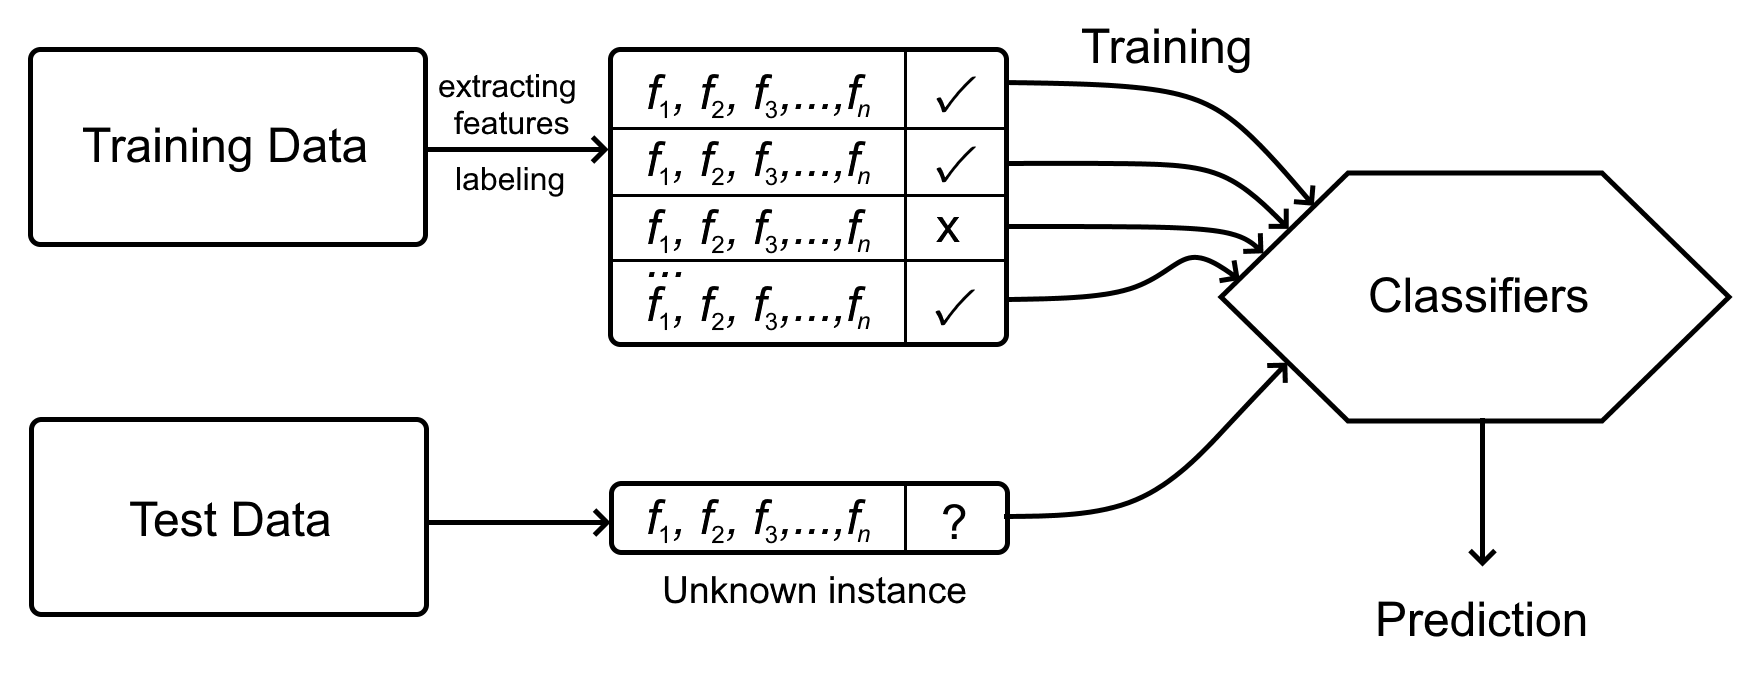
\includegraphics[width=11.5 cm]{f1.png}
\caption{Scheme of the the process of constructing the defect prediction~model.}
\label{fig1} % \label works only AFTER \caption within figure environment
\end{figure}

The survey is structured as follows: Section~\ref{sec_2} briefly describes the methodology of our survey. Section~\ref{sec_3} presents the overview on the various deep learning techniques applied to the defect prediction. In~Section~\ref{sec_4}, we outline the main difficulties of the problem. Section~\ref{sec_5} presents the study of the latest trends in the techniques and methods for defect prediction. Section~\ref{sec_6} concludes the study and offers our vision on the future developments on the~field.

%%%%%%%%%%%%%%%%%%%%%%%%%%%%%%%%%%%%%%%%%%
\section{Methodology}\label{sec_2}

We reviewed the primary studies on the subject. In~this section, we present details of our~methodology.
\pagebreak
\subsection{Research~Questions}

To summarize the work of our survey, let us formulate the following research questions:

\begin{itemize}
\item RQ1. What deep learning techniques have been applied to software defect prediction?
\item RQ2. What are the key factors contributing to the difficulty of the problem?
\item RQ3. What are the trends in the primary studies on the use of deep learning for the software defect prediction?
\end{itemize}

\subsection{Literature Search and Inclusion or Exclusion~Criteria}

To collect related papers, we formulated a search string for Google Scholar and Scopus combining the related keywords ``software engineering'', ``deep learning'', and \mbox{``defect~prediction''.}

To filter the papers with insufficient content and determine the paper quality, we used the following criteria:

\begin{itemize}
\item The paper must describe a technique for automatic feature extraction using deep learning and apply it to the defect prediction problem.
\item The paper length must not be less than six pages.
\end{itemize}


%%%%%%%%%%%%%%%%%%%%%%%%%%%%%%%%%%%%%%%%%%
\section{RQ1. What Techniques Have Been Applied to This Problem?}\label{sec_3}

In order to work with the source code, we need to have its representation.
On the one hand, this representation should be simple as a vector, since most machine learning algorithms work with vectors.
On the other hand, the~representation should contain all the necessary information. 
The numerical vector representing the source code is called an~``embedding''.

There are different ways to represent the source code. Moreover, we need different granularities for different tasks, for example,~for code completion we need token-level embedding and for function clone detection we need function embedding. For~the software defect prediction problem, various levels of granularity are used, such as sub-system, component, file/class, method and~change (see~\cite{AllamanisEtAl2018,ChenMonperrus2019} for more info on various code embeddings).

One way is to create the vector from the hand crafted features.
This approach assumes that an expert invents a set of features and selects best of them (e.g., \cite{SharminEtAl2015,DamEtAl2018}).
Usually, these features include the statistical characteristics of code, such as its size, code complexity, code churn or~process~metrics.

Another way is to create the numerical vector by processing the source~code.

One way to represent the code is a sequence of elements. Usually, they are code tokens or characters~\cite{MikolovEtAl2013}. The~neural networks based on the sequences are usually trained to predict the subsequent~element.

Another approach to build the representation of the source code is the abstract syntax trees (AST)~\cite{ZhangEtAl2019}. The~nodes of the tree correspond to the statement and operators, and~the leaves represent the operands and values. The~tree-based models are trained to predict the code by generating new nodes taking into account the existing tree~structure. 

The most common approach to defect prediction is to use some classification algorithm to divide the source code into two categories: defect code and correct one (e.g.,~\cite{PradelSen2018}).

However, the~approaches based on the hand-crafted features usually do not sufficiently capture the syntax and semantics of the source code. 
Most traditional code metrics cannot distinguish code fragments if these fragments have the same structure and complexity but implement a different functionality.
For example, if~we switch several lines in the code fragments, traditional features, such as the number of lines of code, number of function calls and number of tokens, would remain the same (see~\cite{WangEtAl2016}). Thus, the~semantic information is more important for defect prediction than these~metrics.

Modern approaches are usually based on extracting the implicit structural, syntax and~semantic feature from the source code rather than using the explicit hand-crafted~ones.

The most popular deep learning techniques for software defect prediction are: Deep Belief Networks (DBN), Convolutional Neural Networks (CNN), Long Short Term Memory (LSTM), and~Transformer~architecture.

\subsection{Deep Belief~Networks}

Deep Belief Network~\cite{Bengio2009dbn} generative models are based on a multilevel neural network. This network contains one input layer, one output layer and~multiple hidden layers. The~output layer generates a feature vector representing the data fed to the input layer. Each layer consists of the stochastic nodes. The~important feature of the DBN is that the nodes are only connected to the nodes in the adjacent layers but~not to the nodes within the same layer as shown in Figure~\ref{fig2}.

\begin{figure}[H] %s state preferences regarding figure placement here
% use to correct figure counter if necessary
%\renewcommand{\thefigure}{2}
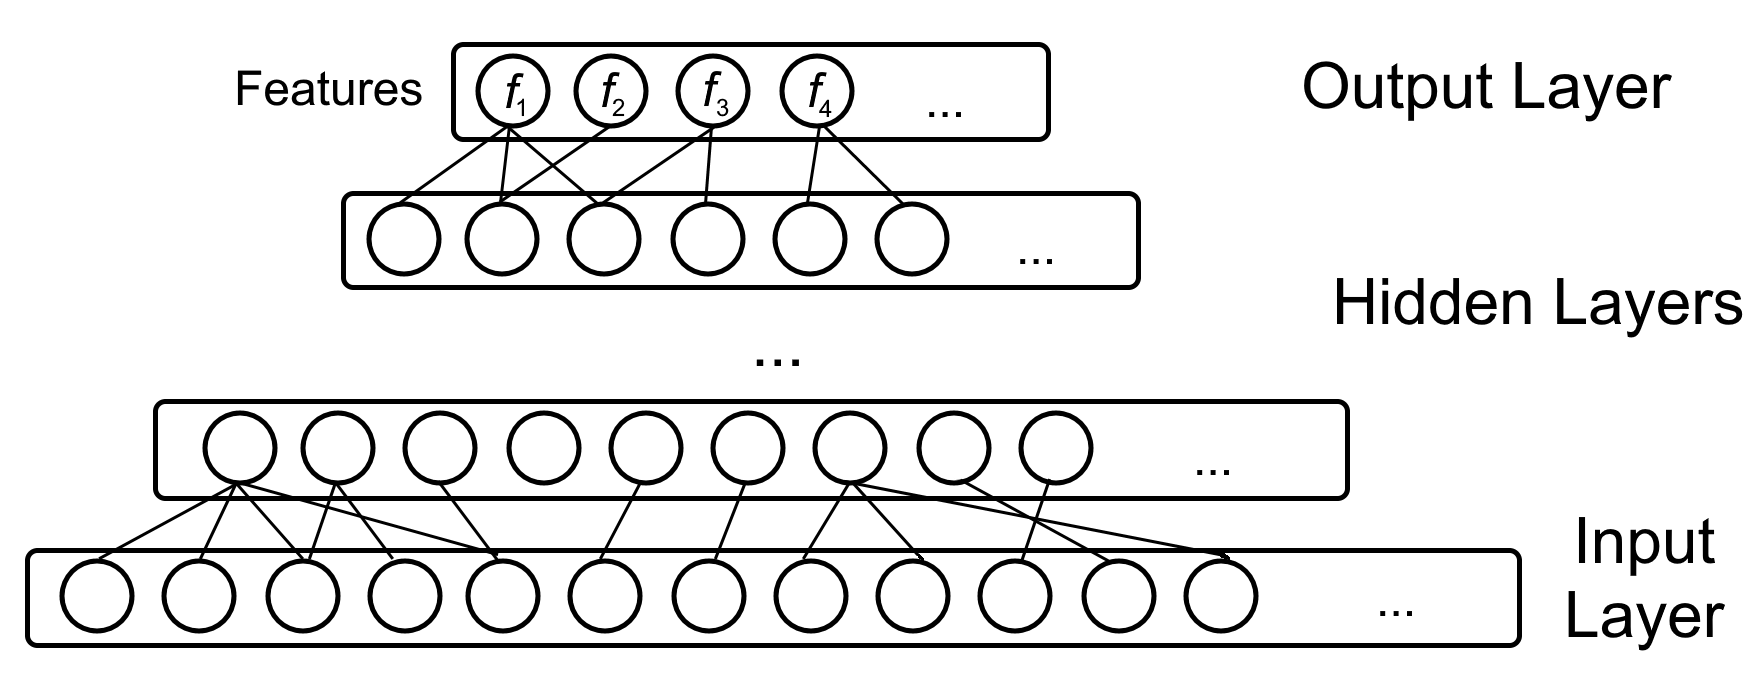
\includegraphics[width=10.5 cm]{f2.png}
\caption{Architecture of the Deep Belief~Network.}
\label{fig2} % \label works only AFTER \caption within figure environment
\end{figure}

Perhaps one of the first works combining AST with the deep learning is~\cite{YangEtAl2015}. The~authors propose the approach for software defect prediction on a changes level. 
The DBN (which is fed by the traditional code metrics) generates the new expressive features and use them in classical machine learning classifiers. 
They extract the relations from the traditional code metrics, such as number of modified modules, directories and~files, added and deleted lines, and~several features related to the developer's experience. Later, the authors proposed the ``TLEL'' approach~\cite{YangEtAl2017} based on the decision tree and ensemble learning for classification. %In the inner layer, it combines decision tree and bagging to build the Random Forest model. In~the outer layer, it uses random under-sampling to train many different Random Forest models and stacking to ensemble them once~more.

The works of Wang~et~al.~\cite{WangEtAl2016, WangEtAl2018} also use the DBN, but~in a different manner.
For predicting the defects on the basis of the code semantics, the~authors have developed a DBN to automatically learn a semantic features from the source code. As~the input for the network, the~programs' AST and source code changes are used for the cases of file-level and change-level prediction, respectively. 
Then, the~authors use the classical machine learning classifiers and extracted features to classify source code files whether they are buggy or~clean.

The main drawback of the DBN is that it does not sufficiently capture the context of the code elements, such as the order of statement execution and function~calls.

\subsection{Long Short Term~Memory}

The Long Short Term Memory~\cite{Hochreiter1997lstm} is a subtype of the recurrent neural network specialized for processing the data sequences. The~LSTM network consists of LSTM units (see Figure~\ref{fig3}). The~key element of the unit is a memory cell, which allows the unit to store the values for a short, as~well as, for~a long time intervals. This provides the LSTM-based models the ability to capture the long-range context information from the source~code.

\begin{figure}[H] %s state preferences regarding figure placement here
% use to correct figure counter if necessary
%\renewcommand{\thefigure}{2}
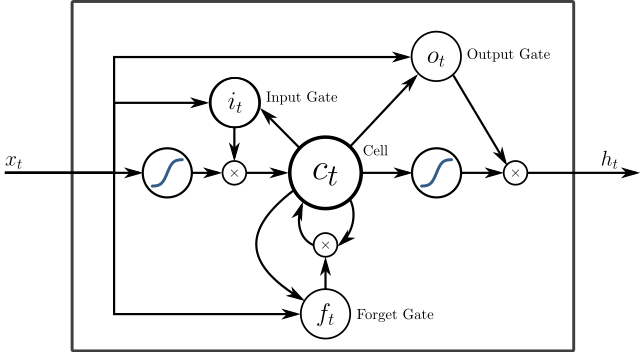
\includegraphics[width=11.5 cm]{f3.png}
\caption{Scheme of the LSTM~unit.}
\label{fig3} % \label works only AFTER \caption within figure environment
\end{figure}


The LSTM-based model was used in work~\cite{DamEtAl2018} for learning both the semantic and syntactic features of code. The~proposed approach represents the code as a sequence of code tokens, which is fed into a LSTM system to transform code into a feature vector and a token state representing the semantic information of the token. Later the Tree-LSTM model was developed using the AST representation as input~\cite{DamEtAl2019}.

A neural bug finding technique is proposed in~\cite{HabibPradel2019}. The~authors train a neural network on examples of the defective and correct code, and~then use the resulting binary classifier for bug detection.
To prepare a labeled dataset, the~authors use the existing static bug detection software to identify the specific kind of bugs.
The code is represented as a tokens sequence and converted to a real-value vector by using the one-hot encoding for each token.
Then, a~bi-directional network with LSTM is used as~model.

In~\cite{ShiEtAl2020}, the~authors propose a model for defect prediction on the base of AST path pair representation.
To process the code, the~path in the AST is extracted as combination of symbol sequence and control sequence. These sequences are fed to a Bi-LSTM network to generate a path vector. Then, all the vectors are combined using the global attention technique to generate the vector for the entire code fragment. These final embedding representations are used for~classification.


\subsection{Convolutional Neural~Networks}

The Convolutional Neural Networks~\cite{Goodfellow-et-al-2016} are a type of neural network specialized for processing the data with a mesh-like structure. This network is characterized by two important features. Firstly, the~local connection pattern between the units is repeated over the entire network. It allows the network to capture the short-term structural context of the source code. Secondly, the~each unit have the same parameters. It allows the network to learn the information on the code element irrespective of its position in the code.
The scheme of general CNN is shown in~Figure~\ref{fig4}.

\begin{figure}[H] %s state preferences regarding figure placement here
% use to correct figure counter if necessary
%\renewcommand{\thefigure}{2}
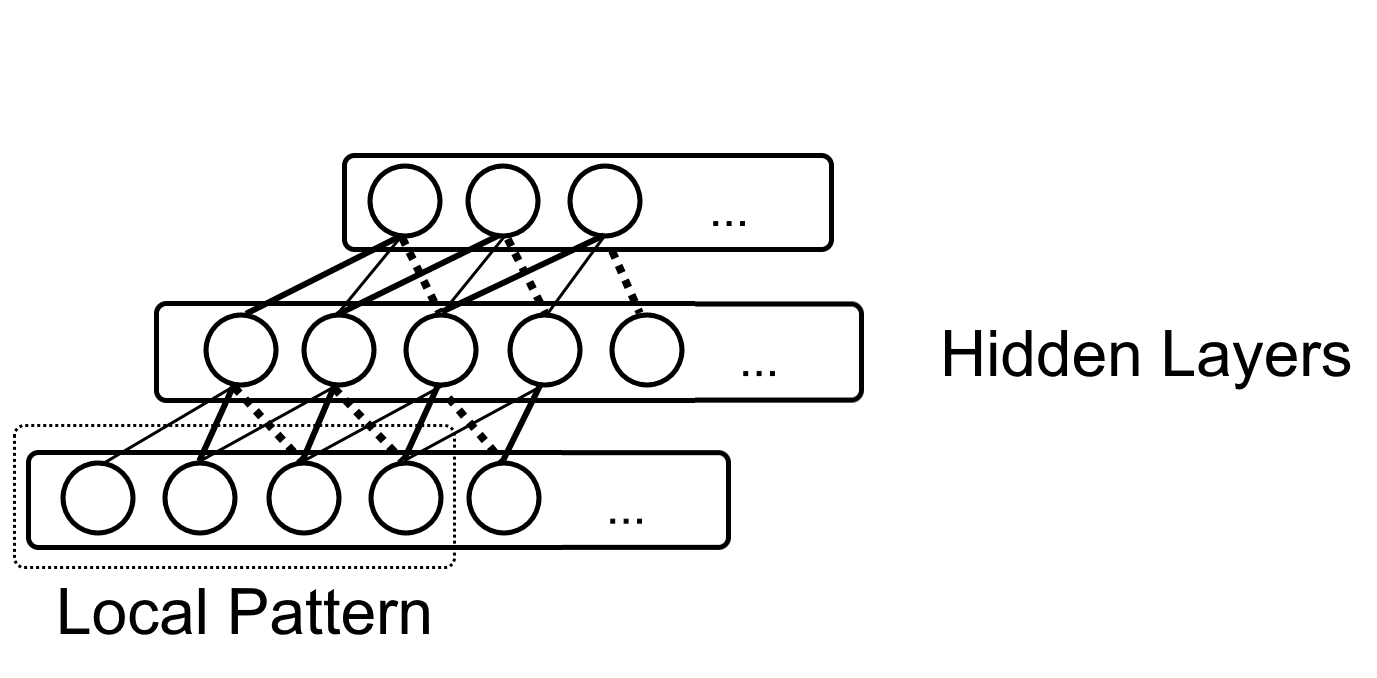
\includegraphics[width=10.5 cm]{f4.png}
\caption{Architecture of the Convolutional Neural~Network.}
\label{fig4} % \label works only AFTER \caption within figure environment
\end{figure}

Reference~\cite{LiEtAl2017} presents the model based on the CNN architecture. Based on the program's AST, the~token vectors are extracted and converted to numerical vectors. Then, these vectors are fed into a CNN. After~that, the~combination of the extracted semantic and structural features and code metrics is used for software defect prediction applying the logistic~regression.

A deep learning model to predict defects on the basis of the commit messages and code changes is developed in~\cite{HoangEtAl2019}. This model is based on the CNN. It uses the convolutional network layers for processing the code changes and commit text and the feature combination layer to fuse these two embedding vectors into a single~one.

Another deep learning-based model for defect prediction is proposed in~\cite{XuEtAl2019}. The~training of the neural network utilizes the triplet loss technique and the weighted cross-entropy loss technique. The~random forest is used as a~classifier.

In~\cite{QiuLuCaiJiang2019}, the~features learning technique based on CNN is proposed. This model extract features from token vectors in the AST of the code and learns the transferable joint features. Combining these deep-learning-generated features with the hand-crafted ones allows the model to perform the cross-project defect prediction. Later, the authors propose a new tree-based convolutional network to perform this task~\cite{CaiLuQiu2019}. It uses the tree-based continuous bag-of-word for encoding the AST nodes to be fed into~CNN.

\subsection{Transformer~Models}

Recently, the~big success of pre-trained contextual representations in the NLP, for example,~\cite{liu2019roberta}, led to a rise of attempts to apply these techniques to source code. Usually, these models are based on the multi-layer Transformer architecture~\cite{vaswani2017attention} shown in \mbox{Figure~\ref{fig5}}. They are pre-trained using the massive unlabeled corpora of programs with the self-supervised objectives, such as masking language modeling and next sentence \mbox{prediction~\cite{KanadeEtAl2019,FengEtAl2020}}. After~the pre-training phase, the~model can be fine-tuned for specific tasks using the supervised~techniques.

\begin{figure}[H] %s state preferences regarding figure placement here
% use to correct figure counter if necessary
%\renewcommand{\thefigure}{2}
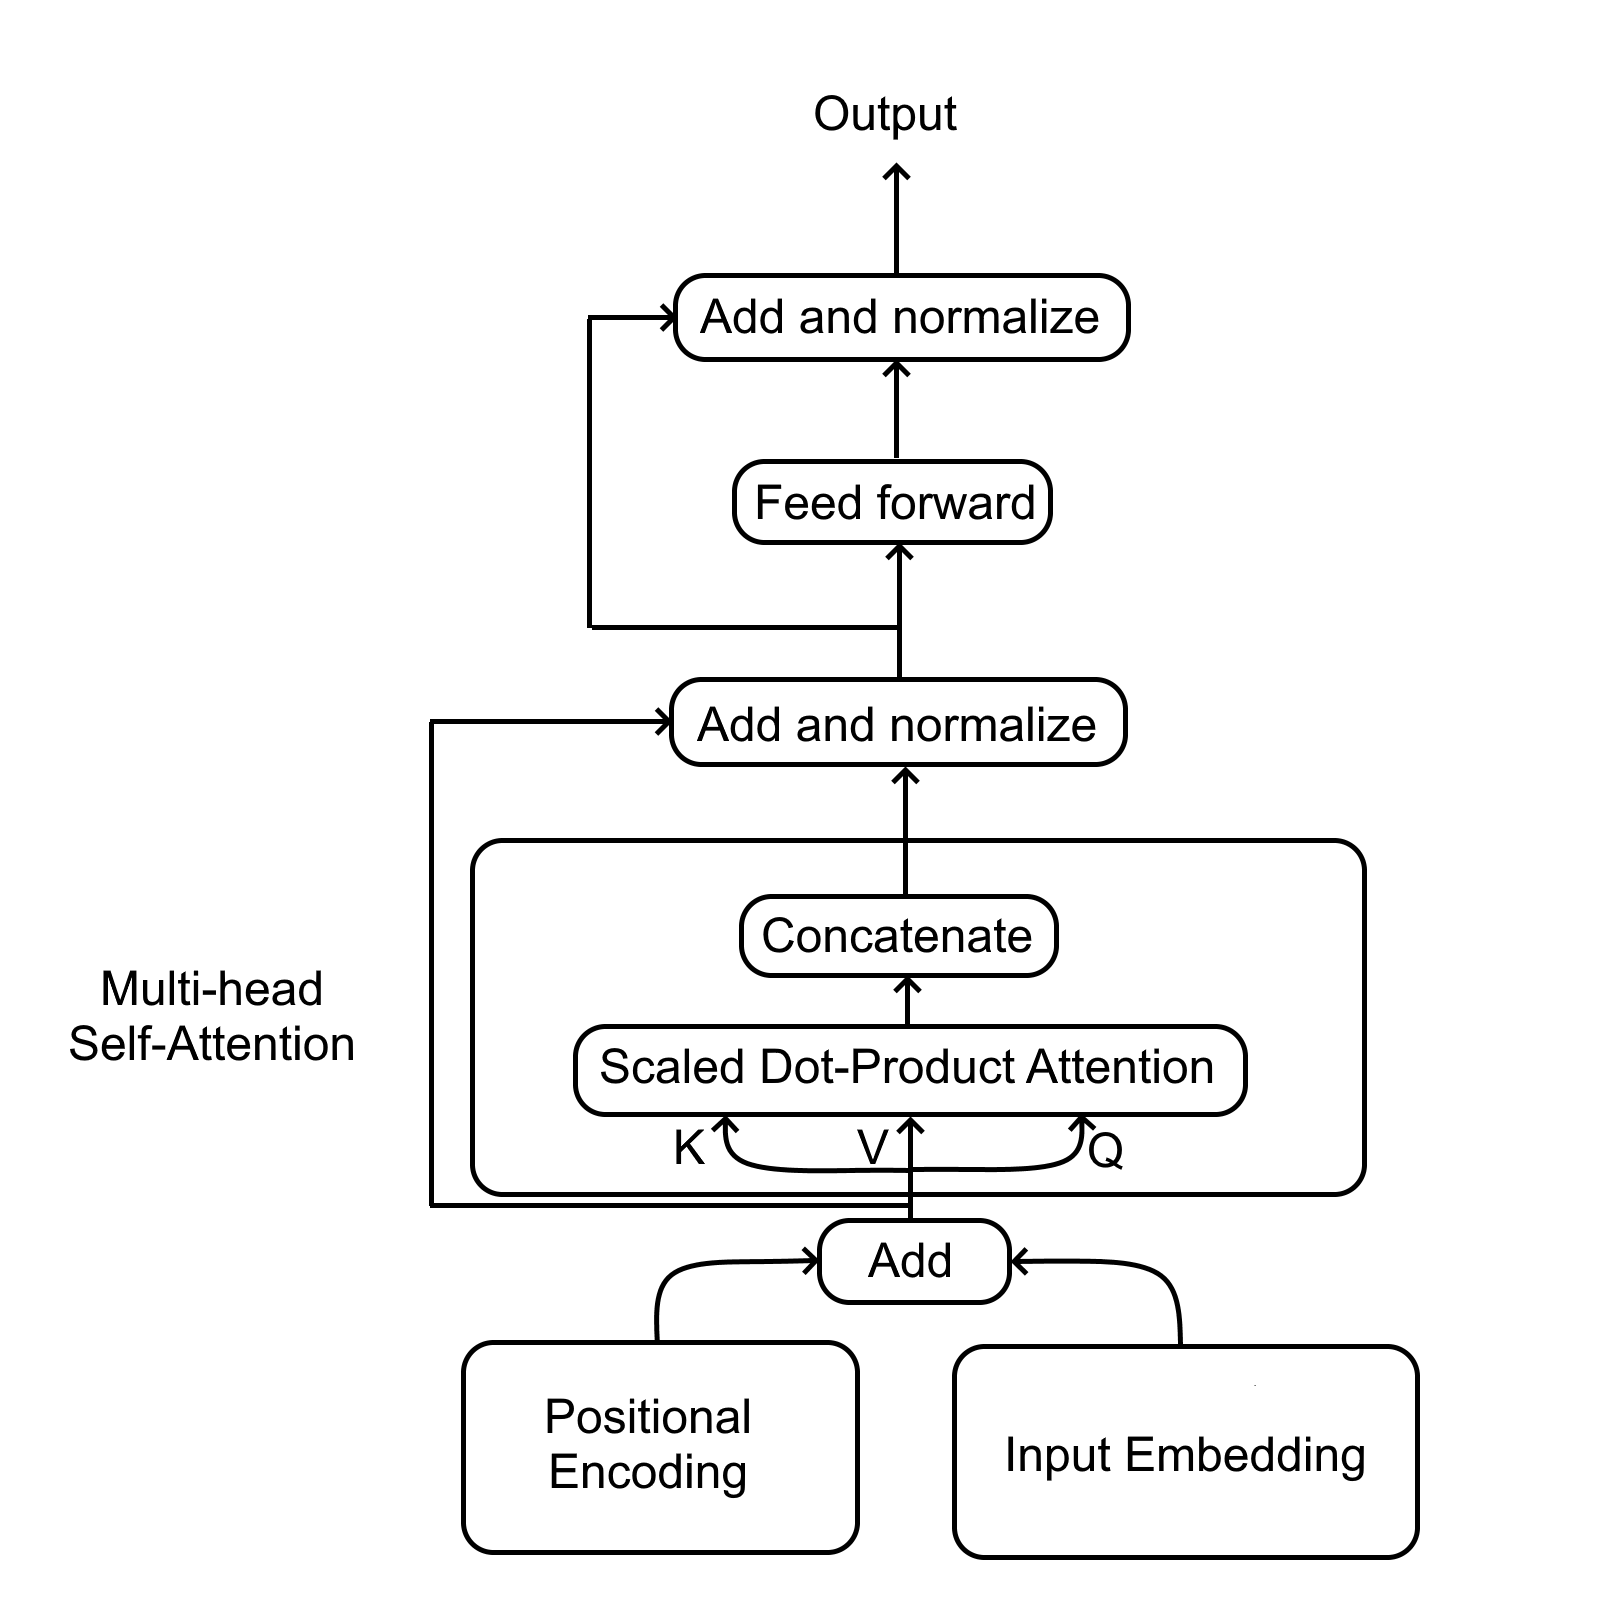
\includegraphics[width=10.5 cm]{f5.png}
\caption{Architecture of the multi-layer~transformer.}
\label{fig5} % \label works only AFTER \caption within figure environment
\end{figure}

The authors of~\cite{HumphreysDam2019} state that the approaches based on the traditional complexity metrics are useless since there is no need for a tool to tell the engineer that longer and more complex code is more defect-prone. The~methods %~\cite{WangEtAl2016} 
of learning features from the source code do not guarantee capturing semantic and syntactical similarity, and~very similar source codes can have very different features. These features can correlate with defects rather than directly cause them.
In contrast, the~authors propose an approach based on the self attention transformer encoder to the semantic defect prediction. The~matrix representing the defectiveness of each token in the fragment is generated. Attention and layer normalization are used as a regularization technique. The~resulting model provides the defect prediction with the semantic highlight of defective code~regions.

The CuBERT model is presented in~\cite{KanadeEtAl2019}. The~authors use a corpus of Python files from the GitHub to create a benchmark for evaluating code embeddings on five classification tasks and a program repair task.
They train their model and compare it with various other models including the BiLSTM and Transformer.
It is shown that the CuBERT outperforms the baseline models~consistently.

A bimodal language model called CodeBERT is presented in~\cite{FengEtAl2020}. It is based on the multilayer bidirectional Transformer neural architecture. To~prepare the data, the~natural language text is represented as a sequence of words, and~the source code is presented as a sequence of tokens.
The output of the CodeBERT model is a contextual vector learned from the natural language and source code, as~well as the~aggregated sequence.
The resulting model efficiently solves the problems of both code to the documentation and natural language code~search. 

Work~\cite{guo2021graphcodebert} presents a multi-layer bidirectional transformer architecture GraphCodeBERT, which utilizes three components as input: the source code, paired comments and~data flow graph. Data flow graph represents relations between variables, for~example, where the value of a variable comes from. This allows the model to consider the code structure for code representation. For~pre-training tasks, the~traditional masked language modeling, as~well as the~edge prediction and node alignment of data flow graph were used.
It supports several downstream code-related tasks including the code clone detection, code translation and~code~refinement.


\subsection{Other~Networks}

In~\cite{TongLiuWang2018}, a~software defect prediction technique based on stacked denoising autoencoders model is presented. The~stacked denoising autoencoder is used to extract higher-level features from the traditional metrics. The~two-stage ensemble learning is used for classification. To~address the class imbalance, the~authors use the ensemble learning strategy. Later, the~feature selection algorithm was applied to this method to address the feature redundancy problem~\cite{TranHanhBinh2019}.

A model for the software defect prediction was constructed in work~\cite{ZhaoEtAl2019} on the base of the Siamese parallel fully-connected networks. This model utilizes the paired parallel Siamese networks architecture and the deep learning approach. The~network produces the high-level features that are used for classification. To~address the imbalance between the minority and majority classes, the~network takes into account the cost-sensitivity~features.

The neural forest networks are used to learn feature representations in~\cite{QiuEtAl2019}. To~perform a classification, a~decision forest is used. It also guides the learning of the neural network. 
In~\cite{ZhouEtAl2019}, a~new deep forest model is proposed for the software defect prediction. 
To detect the essential defect features, it uses the cascade learning strategy, which consists in reforming a set of the random forest classifiers into a layered~network.

The graph neural network to predict the software defects is constructed in work~\cite{XuWangAi2020}. It extracts the semantics and context features from the AST of the code fragments. To~capture the defect-related information from the source code, the~ASTs for the buggy and fixed version of a fragment are constructed and pruned using the community detection algorithm, which extracts the defect-related subtree.
Then, the~Graph Neural Network is used to capture the latent defect~information.


%%%%%%%%%%%%%%%%%%%%%%%%%%%%%%%
\section{RQ2. What Are the Key Factors Contributing to Difficulty of the Problem?} \label{sec_4}

The problem of software defect prediction is considered very complex and very challenging for the machine learning models based on the neural~networks. 

\subsection{Lack of~Data}

One of the difficulties is lack of available large labeled datasets devoted to the defect prediction. To~alleviate this problem, one can utilize the pre-trained contextual embeddings. This technique consists in pre-training the language model on a massive corpora of unlabeled source code using the self-supervised objectives, such as masked language modeling, next sentence prediction and~replaced token~detection. 

Table~\ref{t1} presents the popular unlabeled code datasets suitable for this~task.

% start a new page without indent 4.6cm
%\clearpage
\end{paracol}
\nointerlineskip
\begin{specialtable}[H] \widetable
\caption{List of unlabeled~datasets.\label{t1}}
%%% \tablesize{} %% You can specify the fontsize here, e.g.,~\tablesize{\footnotesize}. If commented out \small will be used.
%\renewcommand{\arraystretch}{2.0}
%\begin{tabular}{cccc}

\begin{tabulary}{\textwidth}{CLLLl}
\toprule
\textbf{Dataset}	& \textbf{Content}	& \textbf{Size}  & \parbox{10em}{\textbf{Used in Tasks}}\\
\midrule
Bigquery github repos~\cite{KanadeEtAl2019} & Python source code & 4 M files & Pre-training CuBERT~model \\
Py150~\cite{RaychevEtAl2016Deep3} & Python source code, AST & 8423 repos, 149,993 files & Fine-tuning CuBERT~model \\
%Variable-Misuse Classification, Wrong Binary Operator, Swapped Operand, Function-Docstring Mismatch, Exception Type, Variable-Misuse Localization and Repair \\
Js150~\cite{RaychevEtAl2016} & Javascript source code, AST & 150,000 source files & Code Summarization; Defect~Prediction\\
Datasets for~\cite{AlonEtAl2019seq} & Java source code & 9500 projects, 16 M samples in the largest one & Code~summarization \\
GitHub Java Corpus~\cite{AllamanisSutton2013} & Java source code & 11,000 projects & Language~Modeling \\
CodeNN Dataset~\cite{IyerEtAl2016} & C\# source code and summaries & 66,015 fragments & Code~Captioning \\
Dataset for~\cite{BryksinEtAl2020} & Kotlin source code, AST, bytecode & 47,751 repos, 932,548 files, 4,044,790 functions & Anomaly detection, defect~prediction \\
Dataset for~\cite{AllamanisBrockschmidtKhademi2018} & C\# source code & 29 projects, 2.9 M lines of code & Variable Misuse~detection \\
\bottomrule
\end{tabulary}
\end{specialtable}
\begin{paracol}{2}
%\linenumbers
\switchcolumn


%Libraries.io & Metadata for software packages & 306k packages & Empirical Comparison of Dependency Network \\
%GHTorrent & GitHub metadata & &	\\


The pre-trained model may then be fine-tuned for the defect prediction using much smaller labeled datasets. Table~\ref{t2} presents a list of publicly available datasets devoted to the defect prediction. Usually, such datasets include pairs of correct and defective code~fragments. 

% start a new page without indent 4.6cm
%\clearpage
\end{paracol}
\nointerlineskip
\begin{specialtable}[H] \widetable
\caption{List of labeled~datasets.\label{t2}}
%%% \tablesize{} %% You can specify the fontsize here, e.g.,~\tablesize{\footnotesize}. If commented out \small will be used.
%\tablesize{\footnotesize}
%\renewcommand{\arraystretch}{2.0}
%\begin{tabular}{cccc}
\begin{tabulary}{\textwidth}{CLLLl}
\toprule
\textbf{Dataset}	& \textbf{Content}	& \textbf{Size}  & \parbox{10em}{\textbf{Used in Tasks}}\\
\midrule
SEIP Lab Software Defect Prediction Data~\cite{mauvsa2016systematic} & Complexity metrics & 5 subsequent releases of 3 projects from the   Java Eclipse community & Data collection and~linking \\
PROMISE Software Engineering Repository~\cite{sayyad2005promise} & Numeric metrics; reported defects (false/true) & 15,000 modules & Defect~prediction \\
NASA Defect Dataset~\cite{shepperd2018nasa} & Numeric metrics; reported defects (false/true) & 51,000 modules & Defect~prediction \\
REPD datasets~\cite{AfricEtAl2020} & Numeric metrics, semantic features, reported defects & 10,885 fragments in the largest one & Defect~prediction \\
GPHR~\cite{XuWangAi2020} & Java code and metrics & 3526 pairs of fragments, buggy and fixed, code metrics & Defect~prediction \\
BugHunter~\cite{FerencEtAl2020} & Java source code; metrics; fix-inducing commit; number of reported bugs & 159 k pairs for 3 granularity levels (file/class/method), 15 projects & Analyzing the importance of complexity~metrics \\
GitHub Bug DataSet~\cite{ferenc2016github_bug} & Java source code; code metrics; number of reported bugs and vulnerabilities & 15 projects; 183 k classes & Bug~prediction \\
Unified Bug Dataset~\cite{ferenc2020public} & Java source code; code metrics; number of reported bugs & 47,618 classes; 43,744 files & Bug~prediction \\
Neural Code Translator Dataset~\cite{TufanoEtAl2018} & Pairs of buggy and fixed abstracted method-level fragments & 46 k pairs of small fragments (under 50 tokens), 50 k pairs of medium fragments (under 100 tokens) & Code~refinement \\
BugsInPy~\cite{WidyasariEtAl2020} & Pair of buggy and fixed Python snippets, manually processed & 493 bugs from 17 projects & Benchmark for testing and debugging~tools \\

Draper VDISC Dataset~\cite{RusselEtAl2018} & C and C++ source code, labeled for potential vulnerabilities & 1.27 M functions & Vulnerability~Detection \\
Refactory Dataset~\cite{yang2019refactory} & Python source code & 2442 correct and 1783 buggy program & Program~repair \\
\hbox{Defect4J}\cite{just2014defects4j} & Java source code & 835 pairs of buggy and fixed fragments & Software testing~research \\
BugSwarm~\cite{Tomassi2019bugswarm} & Java and Python source code & 3232 pairs of buggy and fixed fragments & Software testing~research \\
BuGL~\cite{muvva2020bugl} & C, C++, Java, and~Python source code; issues; pull requests & 54 projects; 151 k closed issues; 10,187 pull requests & Bug~localization \\
Bugs.jar~\cite{SahaEtAl2018bugsjar} & Java source code & 1158 pairs of buggy and and fixed fragments & Program~repair \\
\bottomrule
\end{tabulary}
\end{specialtable}
\begin{paracol}{2}
%\linenumbers
\switchcolumn

As with the other factors affecting the difficulty of constructing datasets, we can highlight that the distribution of the classes in the real code projects is often imbalanced. Usually, there are fewer buggy files or methods in a project than the correct ones. This may lead to the situation where the common classifiers would correctly detect the major class (correct code) and ignore the much smaller class of the defect-prone code.
This will lead to bad performance of the~model.

To address this imbalance, several oversampling methods are proposed. \linebreak In~\cite{AlsawalqahEtAl2017,AgrawalMenzies2018}, the~authors constructed hybrid approaches. It is based on the Synthetic Minority Over-Sampling Technique (SMOTE and SMOTUNED) for preparing the datasets and ensemble approaches for classifying the defective and correct code.
In~\cite{ShiEtAl2020}, the~authors takes into account the proportion of the correct and defective code in each project in the dataset. To~balance the classes, they duplicate the elements of the smaller~class.

\subsection{Lack of~Context}

Another problem is the complexity of the context for the code. Unlike the natural texts, the~code element may depend on another element located far away, maybe, even in another code fragment. Moreover, it is often hard to say if the code element is defective without considering its context. If~dataset consists of the pairs of bugged and fixed code fragments, it is often hard to extract the essence of~defect.

Approaches based on the Transformer networks were aimed to NLP problems where data display a great deal of locality of reference. Most information about a token can be derived from its neighboring tokens~\cite{ tay2020efficient}. Thus, most such models represent the source code as a sequence of~tokens.

The traditional Transformer architectures based on self-attention matrices do not scale well because of quadratic complexity. Usually, they are designed to handle the input sequences with limited length (usually, 512 or 1024 tokens)~\cite{tay2020efficient, tay2020long}.
 Therefore, their applicability to understanding the context of the source code is~limited.
 
There are several modifications to the Transformer architecture that improve its ability to comprehend long sequences~\cite{zaheer2021big,fiok2021text,beltagy2020longformer}. These approaches alleviate the problem of limited length of the input, giving the Transformers the potential to work with a complex context of the source~code. 
 
 Another approach is to capture the structural and global relations on the code, combining the sequence-based and graph-based models for code representation~\cite{hellendoorn2020global,guo2021graphcodebert}. 

Thus, representing the code context is essential in the software defect~prediction. 

%%%%%%%%%%%%%%%%%%%%%%%%%%%%%%%
\section{RQ3. What Are the Trends in the Primary Studies On the Use of Deep Learning for the Software Defect Prediction?} \label{sec_5}

The earliest works, such as~\cite{YangEtAl2015}, utilize the deep learning techniques trying to extract the implicit features from the traditional explicit features (such as code metrics).
The main drawback of this approach is that these traditional features usually cannot capture the semantic difference between the correct and defective code. Therefore, the~combination of these features would also fail to do this~\cite{LiEtAl2017}.

Later approaches~\cite{DamEtAl2019,HoangEtAl2019} use the generic or tailored deep learning techniques to extract the semantic and syntactic features directly from the source code, usually, from~the abstract syntax trees. These deep learned features are used in combination with the traditional ones in the machine classifiers to produce the accurate defect~prediction.

Modern software development often prioritize writing the human-readable source code. This includes using the  meaningful names for the functions and variables and writing the code documentation in natural language. This leads to a situation where we can extract the semantic information from the source code using the techniques originally intended for the NLP, such as the pre-trained language representations such as BERT~\cite{devlin2019bert}. 

Learning useful models with supervised setting is often difficult because labeled data are usually limited. Thus, many unsupervised approaches have been proposed recently to utilize the large unlabeled datasets that are more readily available. Usually, this means that pre-training is performed with automatic supervisions without manual annotation of the samples. Then, the~model may be fine-tuned for the specific task using much smaller supervised data~\cite{KanadeEtAl2019}.

The most recent techniques in software engineering are based on using the general-purposed pre-trained models for programming languages~\cite{karampatsis2020scelmo,guo2021graphcodebert}. These models learn to ``understand'' the source code from unlabeled datasets using the self-supervised objectives. A large corpus of source code is used for pre-training. Usually, the~objective is the Masked Language Modeling where at some positions the tokens are masked out and the model must predict the original token~\cite{FengEtAl2020}. 
Utilizing these techniques alleviates the need for the task-specific architectures and training on large labeled datasets for each task~separately.


%%%%%%%%%%%%%%%%%%%%%%%%%%%%%%%%%%%%%%%%%%
\section{Conclusions} \label{sec_6}

One of the major challenges in modern software engineering is predicting defective code. Recent developments in the field of machine learning, especially the multi-layered neural networks and deep learning algorithms, provide powerful techniques, which utilize learning algorithms for representations of the source code that captures semantic and structural~information. 

This survey presents the latest research progress in software defect prediction using the deep learning techniques, such as the Transformer architectures. We formulate the main difficulties of the defect prediction problem as lack of data and complexity of context and discuss the ways to alleviate these~problems.

Taking into account the latest trends in the machine learning techniques for the software defect prediction problem, we believe that progress in this field will be achieved largely due to the implementation of the following~ideas.
\begin{itemize}
\item To reduce the requirements for the size of the labeled datasets, one should use the self-supervised training on large corpora of the unlabeled data. In~addition, it is necessary to use the unlabeled data for the pre-training of related tasks and to contribute to the fact that the trained models will have a deeper and more comprehensive understanding of the source code. This, in~the turn, will allow one to find the deeper defects.
\item To leverage the latest advances in the machine learning techniques in the natural language processing in the programming languages, we are already seeing the successful migration of these methods to solve various code understanding problems. For~example, optimization of the self-attention mechanism for the transformers will allow one to use them for long sequences, which, in~the turn, will lead to a more complete consideration of the code context for finding the defects.
\item Often a defect is not limited to a single line of code or one function, and~there are various ways to fix it. For~example, a~bug can be fixed either inside the function or at calling this function. Thus, the~defect ceases to have specific coordinates inside the source file. In~addition, not being an explicit defect, a~line of code can become defective at a certain point in time. A~changed context may lead to the fact that the purpose of the code changes, and, therefore, the~old implementation no longer corresponds to the new requirements or specifications. 
\end{itemize}

All this leads to a blurring of the concept of a defect. Thus, we come to the concepts of ``potentially defective'' code or ``strange'' code. In~this regard, as~promising problems, we want to note the task of finding an atypical (or anomalous) code and the task of the code refinement. These task require good representations of the code and code changes, taking into account the specifics of the source code, such as structure and~context.

It is difficult to state which of the state-of-the-art models performs in the best way. There are no universally accepted standard benchmarks for the problem and different researchers utilize different performance metrics and use different data. Thus, the~experimental results from the primary works cannot be directly compared. The~existing comparative studies such as~\cite{Herbold2018benchmark} show that while the state-of-the-art deep learning techniques usually perform better than standard deep learning and traditional metrics-based ones (achieving the increase of F1 from 60\% up to 80\% in some cases). None of the approaches achieves a consistently high performance in terms of recall, precision and~accuracy sufficient for the practical application. Thus, the~defect prediction problem remains an open~one.

%%%%%%%%%%%%%%%%%%%%%%%%%%%%%%%%%%%%%%%%%%
%\section{Patents}

%This section is not mandatory, but may be added if there are patents resulting from the work reported in %this manuscript.

%%%%%%%%%%%%%%%%%%%%%%%%%%%%%%%%%%%%%%%%%%
\vspace{6pt} 

%%%%%%%%%%%%%%%%%%%%%%%%%%%%%%%%%%%%%%%%%%
%% optional
%\supplementary{The following are available online at \linksupplementary{s1}, Figure S1: title, Table S1: title, Video S1: title.}

% Only for the journal Methods and Protocols:
% If you wish to submit a video article, please do so with any other supplementary material.
% \supplementary{The following are available at \linksupplementary{s1}, Figure S1: title, Table S1: title, Video S1: title. A supporting video article is available at doi: link.} 

%%%%%%%%%%%%%%%%%%%%%%%%%%%%%%%%%%%%%%%%%%
\authorcontributions{\hl{Conceptualization, E.N.A., A.V.K.; Methodology, E.N.A., A.V.K, V.E.M.; Investigation, A.Yu.B., A.A.D., K.S.K., A.V.K., I.P.M., V.E.M.; Writing---original draft preparation, V.E.M., Writing---review and editing, E.N.A., K.S.K., A.V.K., V.E.M.; Supervision, E.N.A.}
%All authors (E.N.A., A.Y.B., A.A.D., K.S.K., A.V.K., I.P.M., V.E.M.) contributed equally. 
All authors have read and agreed to the published version of the manuscript.}%please add detailed contributions for all authors, for example:  ``Conceptualization, X.X. and Y.Y.; methodology, X.X.; software, X.X.; validation, X.X., Y.Y. and Z.Z.; formal analysis, X.X.; investigation, X.X.; resources, X.X.; data curation, X.X.; writing---original draft preparation, X.X.; writing---review and editing, X.X.; visualization, X.X.; supervision, X.X.; project administration, X.X.; funding acquisition, Y.Y. All authors have read and agreed to the published version of the manuscript.''
%Authors: We have added the detailed contribution for all authors.

\funding{This research received no external~funding.}
%{Please add: ``This research received no external funding'' or ``This research was funded by NAME OF FUNDER grant number XXX.'' and  and ``The APC was funded by XXX''. Check carefully that the details given are accurate and use the standard spelling of funding agency names at \url{https://search.crossref.org/funding}, any errors may affect your future funding.}

\institutionalreview{\hl{Not applicable.}}%In this section, please add the Institutional Review Board Statement and approval number for studies involving humans or animals. Please note that the Editorial Office might ask you for further information. Please add ``The study was conducted according to the guidelines of the Declaration of Helsinki, and approved by the Institutional Review Board (or Ethics Committee) of NAME OF INSTITUTE (protocol code XXX and date of approval).'' OR ``Ethical review and approval were waived for this study, due to REASON (please provide a detailed justification).'' OR ``Not applicable'' for studies not involving humans or animals. You might also choose to exclude this statement if the study did not involve humans or animals.}
%Authors: Our work does not involve humans or animals.

\informedconsent{\hl{Not applicable.}}%Any research article describing a study involving humans should contain this statement. Please add ``Informed consent was obtained from all subjects involved in the study.'' OR ``Patient consent was waived due to REASON (please provide a detailed justification).'' OR ``Not applicable'' for studies not involving humans. You might also choose to exclude this statement if the study did not involve humans. Written informed consent for publication must be obtained from participating patients who can be identified (including by the patients themselves). Please state ``Written informed consent has been obtained from the patient(s) to publish this paper'' if applicable.}
%Authors: Our work does not involve human patients.

\dataavailability{\hl{No new datasets were created in this survey. The datasets listed in Table~1 and Table~2 are available from their respective authors.}}%In this section, please provide details regarding where data supporting reported results can be found, including links to publicly archived datasets analyzed or generated during the study. Please refer to suggested Data Availability Statements in section ``MDPI Research Data Policies'' at \url{https://www.mdpi.com/ethics}. You might choose to exclude this statement if the study did not report any data.} 
%Authors: We have added the statement on data availability.
%Authors: The source file can't be compiled when we put references like ``Table~\ref{t1}'' instead of ``Table~1'' in this statement.

%\acknowledgments{In this section you can acknowledge any support given which is not covered by the author contribution or funding sections. This may include administrative and technical support, or donations in kind (e.g., materials used for experiments).}

\conflictsofinterest{The authors declare no conflict of~interest. }

%{Declare conflicts of interest or state ``The authors declare no conflict of interest.'' Authors must identify and declare any personal circumstances or interest that may be perceived as inappropriately influencing the representation or interpretation of reported research results. Any role of the funders in the design of the study; in the collection, analyses or interpretation of data; in the writing of the manuscript, or in the decision to publish the results must be declared in this section. If there is no role, please state ``The funders had no role in the design of the study; in the collection, analyses, or interpretation of data; in the writing of the manuscript, or in the decision to publish the~results''.} 

%% Optional
%\sampleavailability{Samples of the compounds ... are available from the authors.}

%%%%%%%%%%%%%%%%%%%%%%%%%%%%%%%%%%%%%%%%%%
%% Only for journal Encyclopedia
%\entrylink{The Link to this entry published on the encyclopedia platform.}

%%%%%%%%%%%%%%%%%%%%%%%%%%%%%%%%%%%%%%%%%%
%% Optional
\abbreviations{Abbreviations}{
The following abbreviations are used in this manuscript:\\

\noindent 
\begin{tabular}{@{}ll}
AST & Abstract Syntax Tree\\
CNN & Convolutional Neural Network\\
DBN & Deep Belief Network\\
DL & Deep Learning\\
LSTM & Long Short Term Memory\\
%ML & Machine Learning\\
NLP & Natural Language Processing\\
SDP & Software Defect Prediction\\
\end{tabular}}

%%%%%%%%%%%%%%%%%%%%%%%%%%%%%%%%%%%%%%%%%%
\end{paracol}
%%%%%%%%%%%%%%%%%%%%%%%%%%%%%%%%%%%%%%%%%%
\reftitle{References}

% Please provide either the correct journal abbreviation (e.g. according to the “List of Title Word Abbreviations” http://www.issn.org/services/online-services/access-to-the-ltwa/) or the full name of the journal.
% Citations and References in Supplementary files are permitted provided that they also appear in the reference list here. 

%=====================================
% References, variant A: external bibliography
%=====================================

%\bibliography{references}
\begin{thebibliography}{999}

\bibitem[iee(2010)]{ieee_standard}
IEEE Standard Classification for Software Anomalies.
\newblock {\em \hl{IEEE Standard 1044-2009 (Revision of IEEE Standard 1044-1993})} {\bf 2010},
  1--23.
  %MDPI: please check and confirm the journal name
  %Authors: It is not a journal, it is a standard by IEEE Organization.
\newblock
  doi:{\changeurlcolor{black}\href{https://doi.org/10.1109/IEEESTD.2010.5399061}{\detokenize{10.1109/IEEESTD.2010.5399061}}}.

\bibitem[{Wang} \em{et~al.}(2016){Wang}, {Liu}, and {Tan}]{WangEtAl2016}
{Wang}, S.; {Liu}, T.; {Tan}, L.
\newblock Automatically Learning Semantic Features for Defect Prediction.
\newblock  In Proceedings of the 2016 IEEE/ACM 38th International Conference on Software Engineering
  (ICSE), \hl{Austin, Texas, USA, 18--20 May 2016}; pp. 297--308,
  %MDPI: please add location (city, country) and date (day month year) of conference
  %Authors: Added.
\newblock
  doi:{\changeurlcolor{black}\href{https://doi.org/10.1145/2884781.2884804}{\detokenize{10.1145/2884781.2884804}}}.

\bibitem[Omri and Sinz(2020)]{OmriSinz2020Survey}
Omri, S.; Sinz, C.
\newblock Deep Learning for Software Defect Prediction: A Survey.
\newblock  In Proceedings of the IEEE/ACM 42nd International Conference on
  Software Engineering \hl{Workshops}; \hl{ICSEW'20; Association for Computing Machinery, 	Seoul, Republic of Korea, 6--11 July 2020}; pp. 209--214,
  %1. MDPI:please add location (city, country) and date (day month year) of conference
  %2. MDPI:has been add like a comment, please check if it is reght?
  %Authors: We have added the correct location and date.
\newblock
  doi:{\changeurlcolor{black}\href{https://doi.org/10.1145/3387940.3391463}{\detokenize{10.1145/3387940.3391463}}}.

\bibitem[Yang \em{et~al.}(2020)Yang, Xia, Lo, and Grundy]{yang2020survey}
Yang, Y.; Xia, X.; Lo, D.; Grundy, J.
\newblock A Survey on Deep Learning for Software Engineering. \emph{arXiv} \textbf{2020}, arXiv:cs.SE/2011.14597.

\bibitem[Shen and Chen(2020)]{ShenChen2020Survey}
Shen, Z.; Chen, S.
\newblock A Survey of Automatic Software Vulnerability Detection, Program
  Repair, and Defect Prediction Techniques.
\newblock {\em Secur. Commun. Networks} {\bf 2020}, {\em
  2020},~8858010,
\newblock
  doi:{\changeurlcolor{black}\href{https://doi.org/10.1155/2020/8858010}{\detokenize{10.1155/2020/8858010}}}.

\bibitem[Bryksin \em{et~al.}(2020)Bryksin, Petukhov, Alexin, Prikhodko,
  Shpilman, Kovalenko, and Povarov]{BryksinEtAl2020}
Bryksin, T.; Petukhov, V.; Alexin, I.; Prikhodko, S.; Shpilman, A.; Kovalenko,
  V.; Povarov, N.
\newblock Using Large-Scale Anomaly Detection on Code to Improve Kotlin
  Compiler.
\newblock  In Proceedings of the 17th International Conference on Mining Software
  \hl{Repositories};  \hl{MSR '20; Association for Computing Machinery, Seoul, Republic of Korea, 29--30 June 2020}; pp. 455–465,
%1. MDPI:please add location and date of conference
%2. MDPI:has been add like a comment
%Authors: We have added the correct location and date.
\newblock
  doi:{\changeurlcolor{black}\href{https://doi.org/10.1145/3379597.3387447}{\detokenize{10.1145/3379597.3387447}}}.

\bibitem[{Phan} and {Le Nguyen}(2017)]{PhanNguyen2017}
{Phan}, A.V.; {Le Nguyen}, M.
\newblock Convolutional neural networks on assembly code for predicting
  software defects.
\newblock  In Proceedings of the 2017 21st Asia Pacific Symposium on Intelligent and Evolutionary
  Systems (IES), \hl{Hanoi, Vietnam, 15--17 November 2017}; pp. 37--42,
%MDPI:please add location (city, country) and date (day month year) of conference
%Authors: We have added the correct location and date.
\newblock
  doi:{\changeurlcolor{black}\href{https://doi.org/10.1109/IESYS.2017.8233558}{\detokenize{10.1109/IESYS.2017.8233558}}}.

\bibitem[Allamanis \em{et~al.}(2018)Allamanis, Barr, Devanbu, and
  Sutton]{AllamanisEtAl2018}
Allamanis, M.; Barr, E.T.; Devanbu, P.; Sutton, C.
\newblock A Survey of Machine Learning for Big Code and Naturalness.
\newblock {\em ACM Comput. Surv.} {\bf 2018}, {\em 51},
\newblock
  doi:{\changeurlcolor{black}\href{https://doi.org/10.1145/3212695}{\detokenize{10.1145/3212695}}}.

\bibitem[Chen and Monperrus(2019)]{ChenMonperrus2019}
Chen, Z.; Monperrus, M.
\newblock A Literature Study of Embeddings on Source Code.  \emph{arXiv} \textbf{2019}, arXiv:cs.LG/1904.03061.

\bibitem[{Sharmin} \em{et~al.}(2015){Sharmin}, {Arefin}, {Wadud}, {Nower}, and
  {Shoyaib}]{SharminEtAl2015}
{Sharmin}, S.; {Arefin}, M.R.; {Wadud}, M.A.; {Nower}, N.; {Shoyaib}, M.
\newblock SAL: An effective method for software defect prediction.
\newblock  In Proceedings of the 2015 18th International Conference on Computer and Information
  Technology (ICCIT), \hl{Dhaka, Bangladesh, 21--23 December 2015}; pp. 184--189,
%MDPI:please add location (city, country) and date (day month year) of conference
%Authors: We have added the correct location and date.
\newblock
  doi:{\changeurlcolor{black}\href{https://doi.org/10.1109/ICCITechn.2015.7488065}{\detokenize{10.1109/ICCITechn.2015.7488065}}}.

\bibitem[{Dam} \em{et~al.}(2018){Dam}, {Tran}, {Pham}, {Ng}, {Grundy}, and
  {Ghose}]{DamEtAl2018}
{Dam}, H.K.; {Tran}, T.; {Pham}, T.; {Ng}, S.W.; {Grundy}, J.; {Ghose}, A.
\newblock Automatic Feature Learning for Predicting Vulnerable Software
  Components.
\newblock {\em IEEE Trans. Softw. Eng.} {\bf 2018}, {\em
  47},~67--85,
\newblock
  doi:{\changeurlcolor{black}\href{https://doi.org/10.1109/TSE.2018.2881961}{\detokenize{10.1109/TSE.2018.2881961}}}.

\bibitem[Mikolov \em{et~al.}(2013)Mikolov, Chen, Corrado, and
  Dean]{MikolovEtAl2013}
Mikolov, T.; Chen, K.; Corrado, G.; Dean, J.
\newblock Efficient Estimation of Word Representations in Vector Space.  \emph{arXiv} \textbf{2013}, arXiv:cs.CL/1301.3781.

\bibitem[{Zhang} \em{et~al.}(2019){Zhang}, {Wang}, {Zhang}, {Sun}, {Wang}, and
  {Liu}]{ZhangEtAl2019}
{Zhang}, J.; {Wang}, X.; {Zhang}, H.; {Sun}, H.; {Wang}, K.; {Liu}, X.
\newblock A Novel Neural Source Code Representation Based on Abstract Syntax
  Tree.
\newblock  In Proceedings of the 2019 IEEE/ACM 41st International Conference on Software Engineering
  (ICSE), \hl{Montreal, QC, Canada, 25--31 May 2019}; pp. 783--794,
%MDPI:please add location (city, country) and date (day month year) of conference
%Authors: We have added the correct location and date.
\newblock
  doi:{\changeurlcolor{black}\href{https://doi.org/10.1109/ICSE.2019.00086}{\detokenize{10.1109/ICSE.2019.00086}}}.

\bibitem[Pradel and Sen(2018)]{PradelSen2018}
Pradel, M.; Sen, K.
\newblock DeepBugs: A Learning Approach to Name-Based Bug Detection.
\newblock {\em Proc. ACM Program. Lang.} {\bf 2018}, {\em 2},
\newblock
  doi:{\changeurlcolor{black}\href{https://doi.org/10.1145/3276517}{\detokenize{10.1145/3276517}}}.

\bibitem[Bengio(2009)]{Bengio2009dbn}
Bengio, Y.
\newblock Learning Deep Architectures for AI.
\newblock {\em Found. Trends Mach. Learn.} {\bf 2009}, {\em 2},~1–127,
\newblock
  doi:{\changeurlcolor{black}\href{https://doi.org/10.1561/2200000006}{\detokenize{10.1561/2200000006}}}.

\bibitem[{Yang} \em{et~al.}(2015){Yang}, {Lo}, {Xia}, {Zhang}, and
  {Sun}]{YangEtAl2015}
{Yang}, X.; {Lo}, D.; {Xia}, X.; {Zhang}, Y.; {Sun}, J.
\newblock Deep Learning for Just-in-Time Defect Prediction.
\newblock  In Proceedings of the 2015 IEEE International Conference on Software Quality, Reliability
  and Security, \hl{Vancouver, BC, Canada, 3--5 August 2015}; pp. 17--26,
\newblock
  doi:{\changeurlcolor{black}\href{https://doi.org/10.1109/QRS.2015.14}{\detokenize{10.1109/QRS.2015.14}}}.
%MDPI:please add location (city, country) and date (day month year) of conference
%Authors: We have added the correct location and date.

\bibitem[Yang \em{et~al.}(2017)Yang, Lo, Xia, and Sun]{YangEtAl2017}
Yang, X.; Lo, D.; Xia, X.; Sun, J.
\newblock TLEL: A two-layer ensemble learning approach for just-in-time defect
  prediction.
\newblock {\em Inf. Softw. Technol.} {\bf 2017}, {\em
  87},~206--220,
\newblock
  doi:{\changeurlcolor{black}\href{https://doi.org/https://doi.org/10.1016/j.infsof.2017.03.007}{\detokenize{10.1016/j.infsof.2017.03.007}}}.

\bibitem[{Wang} \em{et~al.}(2018){Wang}, {Liu}, {Nam}, and {Tan}]{WangEtAl2018}
{Wang}, S.; {Liu}, T.; {Nam}, J.; {Tan}, L.
\newblock Deep Semantic Feature Learning for Software Defect Prediction.
\newblock {\em IEEE Trans. Softw. Eng.} {\bf 2018}, {\em
  46},~1267--1293,
\newblock
  doi:{\changeurlcolor{black}\href{https://doi.org/10.1109/TSE.2018.2877612}{\detokenize{10.1109/TSE.2018.2877612}}}.

\bibitem[Hochreiter and Schmidhuber(1997)]{Hochreiter1997lstm}
Hochreiter, S.; Schmidhuber, J.
\newblock Long Short-Term Memory.
\newblock {\em Neural Comput.} {\bf 1997}, {\em 9},~1735–1780,
\newblock
  doi:{\changeurlcolor{black}\href{https://doi.org/10.1162/neco.1997.9.8.1735}{\detokenize{10.1162/neco.1997.9.8.1735}}}.

\bibitem[{Dam} \em{et~al.}(2019){Dam}, {Pham}, {Ng}, {Tran}, {Grundy}, {Ghose},
  {Kim}, and {Kim}]{DamEtAl2019}
{Dam}, H.K.; {Pham}, T.; {Ng}, S.W.; {Tran}, T.; {Grundy}, J.; {Ghose}, A.;
  {Kim}, T.; {Kim}, C.J.
\newblock Lessons Learned from Using a Deep Tree-Based Model for Software
  Defect Prediction in Practice.
\newblock  In Proceedings of the 2019 IEEE/ACM 16th International Conference on Mining Software
  Repositories (MSR),  \hl{Montreal, QC, Canada, 25--31 May 2019}; pp. 46--57,
  %MDPI:please add location (city, country) and date (day month year) of conference
  %Authors: We have added the correct location and date.
\newblock
  doi:{\changeurlcolor{black}\href{https://doi.org/10.1109/MSR.2019.00017}{\detokenize{10.1109/MSR.2019.00017}}}.

\bibitem[Habib and Pradel(2019)]{HabibPradel2019}
Habib, A.; Pradel, M.
\newblock Neural Bug Finding: A Study of Opportunities and Challenges. \emph{arXiv} \textbf{2019}, arXiv:cs.SE/1906.00307.

\bibitem[Shi \em{et~al.}(2020)Shi, Lu, Chang, and Wei]{ShiEtAl2020}
Shi, K.; Lu, Y.; Chang, J.; Wei, Z.
\newblock PathPair2Vec: An AST path pair-based code representation method for
  defect prediction.
\newblock {\em J. Comput. Lang.} {\bf 2020}, {\em 59},~100979,
\newblock
  doi:{\changeurlcolor{black}\href{https://doi.org/https://doi.org/10.1016/j.cola.2020.100979}{\detokenize{10.1016/j.cola.2020.100979}}}.

\bibitem[Goodfellow \em{et~al.}(2016)Goodfellow, Bengio, and
  Courville]{Goodfellow-et-al-2016}
Goodfellow, I.; Bengio, Y.; Courville, A.
\newblock {\em Deep Learning}; MIT Press: \hl{Cambridge, MA, USA,} %newly added information, please confirm if it is OK? %Authors: the data is correct
  2016.  Available online: 
\newblock \url{http://www.deeplearningbook.org} (\hl{accessed on 17 December 2020}).
%MDPI:please add accessed date (day month year)
%Authors: We have added the access date

\bibitem[{Li} \em{et~al.}(2017){Li}, {He}, {Zhu}, and {Lyu}]{LiEtAl2017}
{Li}, J.; {He}, P.; {Zhu}, J.; {Lyu}, M.R.
\newblock Software Defect Prediction via Convolutional Neural Network.
\newblock In Proceedings of the 2017 IEEE International Conference on Software Quality, Reliability
  and Security (QRS), \hl{Prague, Czech Republic, 25--29 July 2017}; pp. 318--328,
 %MDPI:please add location (city, country) and date (day month year) of conference
 %Authors: We have added the correct location and date.
\newblock
  doi:{\changeurlcolor{black}\href{https://doi.org/10.1109/QRS.2017.42}{\detokenize{10.1109/QRS.2017.42}}}.

\bibitem[{Hoang} \em{et~al.}(2019){Hoang}, {Khanh Dam}, {Kamei}, {Lo}, and
  {Ubayashi}]{HoangEtAl2019}
{Hoang}, T.; {Khanh Dam}, H.; {Kamei}, Y.; {Lo}, D.; {Ubayashi}, N.
\newblock DeepJIT: An End-to-End Deep Learning Framework for Just-in-Time
  Defect Prediction.
\newblock  In Proceedings of the 2019 IEEE/ACM 16th International Conference on Mining Software
  Repositories (MSR), \hl{Montreal, QC, Canada, 25--31 May 2019}, pp. 34--45,
   %MDPI:please add location (city, country) and date (day month year) of conference
   %Authors: We have added the correct location and date.
\newblock
  doi:{\changeurlcolor{black}\href{https://doi.org/10.1109/MSR.2019.00016}{\detokenize{10.1109/MSR.2019.00016}}}.

\bibitem[Xu \em{et~al.}(2019)Xu, Li, Xu, Liu, Luo, Zhang, Zhang, Keung, and
  Tang]{XuEtAl2019}
Xu, Z.; Li, S.; Xu, J.; Liu, J.; Luo, X.; Zhang, Y.; Zhang, T.; Keung, J.;
  Tang, Y.
\newblock LDFR: Learning deep feature representation for software defect
  prediction.
\newblock {\em J. Syst. Softw.} {\bf 2019}, {\em 158},~110402,
\newblock
  doi:{\changeurlcolor{black}\href{https://doi.org/https://doi.org/10.1016/j.jss.2019.110402}{\detokenize{10.1016/j.jss.2019.110402}}}.

\bibitem[Qiu \em{et~al.}()Qiu, Lu, Cai, and Jiang]{QiuLuCaiJiang2019}
Qiu, S.; Lu, L.; Cai, Z.; Jiang, S.
\newblock \emph{Cross-Project Defect Prediction Via Transferable Deep
  Learning-Generated and Handcrafted \hl{Features}}.
\newblock  \hl{In Proceedings of The 31st International Conference on Software Engineering \& Knowledge Engineering (SEKE 2019)}, \hl{Lisbon, Portugal, 10-12 July 2019}, pp. 1--6,
Available online: 
\newblock \url{http://ksiresearch.org/seke/seke19paper/seke19paper_70.pdf} (\hl{accessed on 17 December 2020}).
%MDPI: please add publisher, publisher location and year
%Authors: We have added the information for this citation

\bibitem[{Cai} \em{et~al.}(2019){Cai}, {Lu}, and {Qiu}]{CaiLuQiu2019}
{Cai}, Z.; {Lu}, L.; {Qiu}, S.
\newblock An Abstract Syntax Tree Encoding Method for Cross-Project Defect
  Prediction.
\newblock {\em IEEE Access} {\bf 2019}, {\em 7},~170844--170853,
\newblock
  doi:{\changeurlcolor{black}\href{https://doi.org/10.1109/ACCESS.2019.2953696}{\detokenize{10.1109/ACCESS.2019.2953696}}}.

\bibitem[Liu \em{et~al.}(2019)Liu, Ott, Goyal, Du, Joshi, Chen, Levy, Lewis,
  Zettlemoyer, and Stoyanov]{liu2019roberta}
Liu, Y.; Ott, M.; Goyal, N.; Du, J.; Joshi, M.; Chen, D.; Levy, O.; Lewis, M.;
  Zettlemoyer, L.; Stoyanov, V.
\newblock RoBERTa: A Robustly Optimized BERT Pretraining Approach.  \emph{arXiv} \textbf{2019}, arXiv:cs.CL/1907.11692.

\bibitem[Vaswani \em{et~al.}(2017)Vaswani, Shazeer, Parmar, Uszkoreit, Jones,
  Gomez, Kaiser, and Polosukhin]{vaswani2017attention}
Vaswani, A.; Shazeer, N.; Parmar, N.; Uszkoreit, J.; Jones, L.; Gomez, A.N.;
  Kaiser, L.; Polosukhin, I.
\newblock Attention Is All You Need.  \emph{arXiv} \textbf{2017}, arXiv:cs.CL/1706.03762.

%\bibitem[Kanade \em{et~al.}(2020)Kanade, Maniatis, Balakrishnan, and
%  Shi]{KanadeEtAl2019}
%\hl{Kanade, A.; Maniatis, P.; Balakrishnan, G.; Shi, K.} 
%\newblock Learning and Evaluating Contextual Embedding of Source Code. \emph{arXiv} \textbf{2020}, arXiv:cs.SE/2001.00059.  
%MDPI:  ref 31 and ref 41 are in same authors and title, please  confirm if they are duplicate? if yes, please revise. if not, please explain.
%Authors: revised, removed the duplicate reference. The correct entry is below:
\bibitem[Kanade \em{et~al.}(2020)Kanade, Maniatis, Balakrishnan, and
  Shi]{KanadeEtAl2019}
\hl{Kanade, A.; Maniatis, P.; Balakrishnan, G.; Shi, K.}
\newblock Learning and Evaluating Contextual Embedding of Source Code.
\newblock  In \emph{Proceedings
  of Machine Learning Research, Proceedings of the 37th International Conference on Machine
  \hl{Learning, Virtual Event, 13--18 July 2020}}; \hl{Daum\'{e}~III,~H.}; Singh, A., Eds.; PMLR:  \hl{2020}; Volume 119, pp. 5110--5121.
%MDPI:please add location (city, country) and date (day month year) of conference
%Authors: added correct information
%MDPI: incorrect editor name, please check and revise it
%Authors: corrected editor's name
%MDPI: please add lcoation of publisher
%Authors: It is an electronic publisher. We can't find any references to their location.

\bibitem[Feng \em{et~al.}(2020)Feng, Guo, Tang, Duan, Feng, Gong, Shou, Qin,
  Liu, Jiang, and Zhou]{FengEtAl2020}
Feng, Z.; Guo, D.; Tang, D.; Duan, N.; Feng, X.; Gong, M.; Shou, L.; Qin, B.;
  Liu, T.; Jiang, D.; et al.
\newblock CodeBERT: A Pre-Trained Model for Programming and Natural Languages. \emph{arXiv} \textbf{2020}, arXiv:cs.CL/2002.08155.

\bibitem[Humphreys and Dam(2019)]{HumphreysDam2019}
Humphreys, J.; Dam, H.K.
\newblock An Explainable Deep Model for Defect Prediction.
\newblock  In Proceedings of the 22019 IEEE/ACM 7th International Workshop on Realizing Artificial Intelligence Synergies in Software Engineering (RAISE), \hl{Montreal, QC, Canada, 28 May 2019}, pp. 49--55,
\newblock
  doi:{\changeurlcolor{black}\href{https://doi.org/10.1109/RAISE.2019.00016}{\detokenize{10.1109/RAISE.2019.00016}}}.
%MDPI:please add location (city, country) and date (day month year) of conference
%MDPI: please add  publisher location 
%Authors: we have added the correct information

\bibitem[Guo \em{et~al.}(2021)Guo, Ren, Lu, Feng, Tang, Liu, Zhou, Duan,
  Svyatkovskiy, Fu, Tufano, Deng, Clement, Drain, Sundaresan, Yin, Jiang, and
  Zhou]{guo2021graphcodebert}
Guo, D.; Ren, S.; Lu, S.; Feng, Z.; Tang, D.; Liu, S.; Zhou, L.; Duan, N.;
  Svyatkovskiy, A.; Fu, S.; et al.
\newblock GraphCodeBERT: Pre-training Code Representations with Data Flow.
\emph{arXiv} \textbf{2021},  arXiv:cs.SE/2009.08366.

\bibitem[Tong \em{et~al.}(2018)Tong, Liu, and Wang]{TongLiuWang2018}
Tong, H.; Liu, B.; Wang, S.
\newblock Software defect prediction using stacked denoising autoencoders and
  two-stage ensemble learning.
\newblock {\em Inf. Softw. Technol.} {\bf 2018}, {\em
  96},~94--111,
\newblock
  doi:{\changeurlcolor{black}\href{https://doi.org/https://doi.org/10.1016/j.infsof.2017.11.008}{\detokenize{10.1016/j.infsof.2017.11.008}}}.

\bibitem[{Tran} \em{et~al.}(2019){Tran}, {Hanh}, and {Binh}]{TranHanhBinh2019}
{Tran}, H.D.; {Hanh}, L.T.M.; {Binh}, N.T.
\newblock Combining feature selection, feature learning and ensemble learning
  for software fault prediction.
\newblock  In Proceedings of the 2019 11th International Conference on Knowledge and Systems
  Engineering (KSE), \hl{Da Nang, Vietnam, 24--26 October 2019}; pp. 1--8,
%MDPI:please add location (city, country) and date (day month year) of conference
%Authors: We have added correct information.
\newblock
  doi:{\changeurlcolor{black}\href{https://doi.org/10.1109/KSE.2019.8919292}{\detokenize{10.1109/KSE.2019.8919292}}}.

\bibitem[Zhao \em{et~al.}(2019)Zhao, Shang, Zhao, Zhang, and
  Tang]{ZhaoEtAl2019}
Zhao, L.; Shang, Z.; Zhao, L.; Zhang, T.; Tang, Y.Y.
\newblock Software defect prediction via cost-sensitive Siamese parallel
  fully-connected neural networks.
\newblock {\em Neurocomputing} {\bf 2019}, {\em 352},~64--74,
\newblock
  doi:{\changeurlcolor{black}\href{https://doi.org/https://doi.org/10.1016/j.neucom.2019.03.076}{\detokenize{10.1016/j.neucom.2019.03.076}}}.

\bibitem[{Qiu} \em{et~al.}(2019){Qiu}, {Liu}, {Liu}, {Zhu}, and
  {Xu}]{QiuEtAl2019}
{Qiu}, Y.; {Liu}, Y.; {Liu}, A.; {Zhu}, J.; {Xu}, J.
\newblock Automatic Feature Exploration and an Application in Defect
  Prediction.
\newblock {\em IEEE Access} {\bf 2019}, {\em 7},~112097--112112,
\newblock
  doi:{\changeurlcolor{black}\href{https://doi.org/10.1109/ACCESS.2019.2934530}{\detokenize{10.1109/ACCESS.2019.2934530}}}.

\bibitem[Zhou \em{et~al.}(2019)Zhou, Sun, Xia, Li, and Chen]{ZhouEtAl2019}
Zhou, T.; Sun, X.; Xia, X.; Li, B.; Chen, X.
\newblock Improving defect prediction with deep forest.
\newblock {\em Inf. Softw. Technol.} {\bf 2019}, {\em
  114},~204--216,
\newblock
  doi:{\changeurlcolor{black}\href{https://doi.org/https://doi.org/10.1016/j.infsof.2019.07.003}{\detokenize{10.1016/j.infsof.2019.07.003}}}.

\bibitem[{Xu} \em{et~al.}(2020){Xu}, {Wang}, and {Ai}]{XuWangAi2020}
{Xu}, J.; {Wang}, F.; {Ai}, J.
\newblock Defect Prediction With Semantics and Context Features of Codes Based
  on Graph Representation Learning.
\newblock {\em IEEE Trans. Reliab.} {\bf 2020}, 1--13,
\newblock
  doi:{\changeurlcolor{black}\href{https://doi.org/10.1109/TR.2020.3040191}{\detokenize{10.1109/TR.2020.3040191}}}.

%Authors: removed duplicate entry, the correct version is {KanadeEtAl2019} [31]
%\bibitem[Kanade \em{et~al.}(2020)Kanade, Maniatis, Balakrishnan, and
%  Shi]{kanade20cubert}
%\hl{Kanade, A.; Maniatis, P.; Balakrishnan, G.; Shi, K.}
%\newblock Learning and Evaluating Contextual Embedding of Source Code.
%\newblock  In \emph{Proceedings
%  of Machine Learning Research, Proceedings of the 37th International Conference on Machine
%  \hl{Learning}}; \hl{III, H.D.}; Singh, A., Eds.; PMLR:  \hl{2020}; Volume 119, pp. 5110--5121.
%MDPI:please add location (city, country) and date (day month year) of conference
%MDPI: incorrect editor name, please check and revise it
%MDPI: please add lcoation of publisher

\bibitem[Raychev \em{et~al.}(2016{\natexlab{a}})Raychev, Bielik, and
  Vechev]{RaychevEtAl2016Deep3}
Raychev, V.; Bielik, P.; Vechev, M.
\newblock Probabilistic Model for Code with Decision Trees.
\newblock {\em SIGPLAN Not.} {\bf 2016}, {\em 51},~731–747,
\newblock
  doi:{\changeurlcolor{black}\href{https://doi.org/10.1145/3022671.2984041}{\detokenize{10.1145/3022671.2984041}}}.

\bibitem[Raychev \em{et~al.}(2016{\natexlab{b}})Raychev, Bielik, Vechev, and
  Krause]{RaychevEtAl2016}
Raychev, V.; Bielik, P.; Vechev, M.; Krause, A.
\newblock Learning Programs from Noisy Data.
\newblock {\em SIGPLAN Not.} {\bf 2016}, {\em 51},~761--774,
\newblock
  doi:{\changeurlcolor{black}\href{https://doi.org/10.1145/2914770.2837671}{\detokenize{10.1145/2914770.2837671}}}.

\bibitem[Alon \em{et~al.}(2019)Alon, Brody, Levy, and Yahav]{AlonEtAl2019seq}
Alon, U.; Brody, S.; Levy, O.; Yahav, E.
\newblock code2seq: Generating Sequences from Structured Representations of
  Code. \emph{arXiv} \textbf{2019}, arXiv:cs.LG/1808.01400.

\bibitem[{Allamanis} and {Sutton}(2013)]{AllamanisSutton2013}
{Allamanis}, M.; {Sutton}, C.
\newblock Mining source code repositories at massive scale using language
  modeling.
\newblock In Proceedings of the 2013 10th Working Conference on Mining Software Repositories (MSR),
  \hl{San Francisco, CA, USA, 18--19 May 2013}; pp. 207--216,
 %MDPI:please add location and date of conference
 %Authors: We have added location and date.
\newblock
  doi:{\changeurlcolor{black}\href{https://doi.org/10.1109/MSR.2013.6624029}{\detokenize{10.1109/MSR.2013.6624029}}}.

\bibitem[Iyer \em{et~al.}(2016)Iyer, Konstas, Cheung, and
  Zettlemoyer]{IyerEtAl2016}
Iyer, S.; Konstas, I.; Cheung, A.; Zettlemoyer, L.
\newblock Summarizing source code using a neural attention model.
\newblock In Proceedings of the 54th Annual Meeting of the Association for
  Computational Linguistics (Volume 1: Long Papers), \hl{Berlin, Germany, 7--12 August 2016}; pp. 2073--2083.
%MDPI:please add location and date of conference
%Authors: added location and date.

\bibitem[Allamanis \em{et~al.}(2018)Allamanis, Brockschmidt, and
  Khademi]{AllamanisBrockschmidtKhademi2018}
Allamanis, M.; Brockschmidt, M.; Khademi, M.
\newblock Learning to Represent Programs with Graphs. \emph{arXiv} \textbf{2018},
arXiv:cs.LG/1711.00740.

\bibitem[Mau{\v{s}}a \em{et~al.}(2016)Mau{\v{s}}a, Galinac-Grbac, and
  Dalbelo-Ba{\v{s}}i{\'c}]{mauvsa2016systematic}
Mau{\v{s}}a, G.; Galinac-Grbac, T.; Dalbelo-Ba{\v{s}}i{\'c}, B.
\newblock A systematic data collection procedure for software defect
  prediction.
\newblock {\em Comput. Sci. Inf. Syst.} {\bf 2016}, {\em
  13},~173--197.

\bibitem[Sayyad~Shirabad and Menzies(2005)]{sayyad2005promise}
Sayyad~Shirabad, J.; Menzies, T.
\newblock {The {PROMISE} Repository of Software Engineering \hl{Databases}.}
\newblock School of Information Technology and Engineering, University of
  Ottawa, \hl{Canada},  2005,
Available online: 
\newblock \url{http://promise.site.uottawa.ca/SERepository/} (\hl{accessed on 17 December 2020}).
%Please indicate the level of thesis (Bachelor’s Thesis, Master’s Thesis, Ph.D. Thesis…).
%please add lcoation of university
%Authors: It is a reference to the Online resource, not a thesis. 

\bibitem[Shepperd \em{et~al.}(2018)Shepperd, SOng, Sun, and
  Mair]{shepperd2018nasa}
Shepperd, M.; Song, Q.; Sun, Z.; Mair, C.
\newblock NASA MDP Software Defects Data Sets.  \textbf{\hl{2018}}, Available online: 
%MDPI:Please add journal name
%Authors: It is not a journal, it is the online resource with DOI.
\newblock \url{https://doi.org/10.6084/m9.figshare.c.4054940.v1}
(\hl{accessed on 17 December 2020}).

\bibitem[Afric \em{et~al.}(2020)Afric, Sikic, Kurdija, and
  Silic]{AfricEtAl2020}
Afric, P.; Sikic, L.; Kurdija, A.S.; Silic, M.
\newblock REPD: Source code defect prediction as anomaly detection.
\newblock {\em J. Syst. Softw.} {\bf 2020}, {\em 168},~110641,
\newblock
  doi:{\changeurlcolor{black}\href{https://doi.org/https://doi.org/10.1016/j.jss.2020.110641}{\detokenize{10.1016/j.jss.2020.110641}}}.

%\bibitem[Fei \em{et~al.}(2020)Fei, Jun, and Jiaxi]{ghpr2020}
%Fei, W.; Jun, A.; Jiaxi, X.
%\newblock Software Defect Prediction Based on Graph Representation Learning.
%\newblock {\em IEEE Trans. Softw. Eng.} {\bf \hl{2020}}.
%MDPI: Please add volume and page number
%Authors: This reference was a duplicate of {XuWangAi2020} [40]. 

\bibitem[Ferenc \em{et~al.}(2020)Ferenc, Gyimesi, Gyimesi, Tóth, and
  Gyimóthy]{FerencEtAl2020}
Ferenc, R.; Gyimesi, P.; Gyimesi, G.; Tóth, Z.; Gyimóthy, T.
\newblock An automatically created novel bug dataset and its validation in bug
  prediction.
\newblock {\em J. Syst. Softw.} {\bf 2020}, {\em 169},~110691,
\newblock
  doi:{\changeurlcolor{black}\href{https://doi.org/https://doi.org/10.1016/j.jss.2020.110691}{\detokenize{10.1016/j.jss.2020.110691}}}.

\bibitem[T{\'o}th \em{et~al.}(2016)T{\'o}th, Gyimesi, and
  Ferenc]{ferenc2016github_bug}
T{\'o}th, Z.; Gyimesi, P.; Ferenc, R.
\newblock A Public Bug Database of GitHub Projects and Its Application in Bug
  Prediction.
\newblock   In Proceedings of the Computational Science and Its Applications --- ICCSA, \hl{Beijing, China, 4--7 July 2016}; Springer
  International Publishing: Cham,  Switzerland, 2016; pp. 625--638,
\newblock
  doi:{\changeurlcolor{black}\href{https://doi.org/https://doi.org/10.1007/978-3-319-42089-9_44}{\detokenize{10.1007/978-3-319-42089-9_44}}}.
%MDPI:please add location (city, country) and date (day month year) of conference
%Authors: we have added location, date, and DOI link.

\bibitem[Ferenc \em{et~al.}(2020)Ferenc, T{\'o}th, Lad{\'a}nyi, Siket, and
  Gyim{\'o}thy]{ferenc2020public}
Ferenc, R.; T{\'o}th, Z.; Lad{\'a}nyi, G.; Siket, I.; Gyim{\'o}thy, T.
\newblock A public unified bug dataset for java and its assessment regarding
  metrics and bug prediction.
\newblock {\em Softw. Qual. J.} {\bf 2020}, {\em \hl{28}},~\hl{1447--1506},
\newblock
  doi:{\changeurlcolor{black}\href{https://doi.org/https://doi.org/10.1007/s11219-020-09515-0}{\detokenize{10.1007/s11219-020-09515-0}}}.
%MDPI: Please add volume number
%Authors: Added volume number, DOI link, corrected pages.

\bibitem[Tufano \em{et~al.}(2018)Tufano, Watson, Bavota, Penta, White, and
  Poshyvanyk]{TufanoEtAl2018}
Tufano, M.; Watson, C.; Bavota, G.; Penta, M.D.; White, M.; Poshyvanyk, D.
\newblock An Empirical Study on Learning Bug-Fixing Patches in the Wild via
  Neural Machine Translation.
\newblock {\em \hl{ACM Trans. Softw. Eng. Methodol.}} {\bf \hl{2019}}, {\em \hl{28(4)}},~\hl{4:1--4:29},
\newblock
  doi:{\changeurlcolor{black}\href{https://doi.org/https://doi.org/10.1145/3340544}{\detokenize{10.1145/3340544}}}.
%MDPI: Please add volume number
%Authors: Corrected the reference.

\bibitem[Widyasari \em{et~al.}(2020)Widyasari, Sim, Lok, Qi, Phan, Tay, Tan,
  Wee, Tan, Yieh, Goh, Thung, Kang, Hoang, Lo, and Ouh]{WidyasariEtAl2020}
Widyasari, R.; Sim, S.Q.; Lok, C.; Qi, H.; Phan, J.; Tay, Q.; Tan, C.; Wee, F.;
  Tan, J.E.; Yieh, Y.; et al.
\newblock BugsInPy: a database of existing bugs in Python programs to enable
  controlled testing and debugging studies.
\newblock In Proceedings of the {ESEC/FSE} '20: 28th {ACM} Joint European Software Engineering
  Conference and Symposium on the Foundations of Software Engineering, Virtual
  Event, USA, 8--13 November 2020; Devanbu, P., Cohen, M.B., Zimmermann, T.,
  Eds.; {ACM}:  \hl{New York, NY, USA, 2020}; pp. 1556--1560,
  %MDPI: please add location (cith country) of publisher
  %Authors: added location.
\newblock
  doi:{\changeurlcolor{black}\href{https://doi.org/10.1145/3368089.3417943}{\detokenize{10.1145/3368089.3417943}}}.

\bibitem[{Russell} \em{et~al.}(2018){Russell}, {Kim}, {Hamilton}, {Lazovich},
  {Harer}, {Ozdemir}, {Ellingwood}, and {McConley}]{RusselEtAl2018}
{Russell}, R.; {Kim}, L.; {Hamilton}, L.; {Lazovich}, T.; {Harer}, J.;
  {Ozdemir}, O.; {Ellingwood}, P.; {McConley}, M.
\newblock Automated Vulnerability Detection in Source Code Using Deep
  Representation Learning.
\newblock In Proceedings of the 2018 17th IEEE International Conference on Machine Learning and
  Applications (ICMLA),  \hl{Orlando, FL, USA, 17-20 December 2018}; pp. 757--762,
%MDPI:please add location (city, country) and date (day month year) of conference
%Authors: added location and date.
\newblock
  doi:{\changeurlcolor{black}\href{https://doi.org/10.1109/ICMLA.2018.00120}{\detokenize{10.1109/ICMLA.2018.00120}}}.

\bibitem[Hu \em{et~al.}(2019)Hu, Ahmed, Mechtaev, Leong, and
  Roychoudhury]{yang2019refactory}
Hu, Y.; Ahmed, U.Z.; Mechtaev, S.; Leong, B.; Roychoudhury, A.
\newblock Re-factoring based Program Repair applied to Programming Assignments.
\newblock In Proceedings of the 2019 34th IEEE/ACM International Conference on Automated Software
  Engineering (ASE), IEEE/ACM,  \hl{San Diego, CA, USA, 11-15 November 2019}; pp. 388--398,
\newblock
  doi:{\changeurlcolor{black}\href{https://doi.org/10.1109/ASE.2019.00044}{\detokenize{10.1109/ASE.2019.00044}}}.
%MDPI:please add location (city, country) and date (day month year) of conference
%Authors:added location and date and DOI link

\bibitem[Just \em{et~al.}(2014)Just, Jalali, and Ernst]{just2014defects4j}
Just, R.; Jalali, D.; Ernst, M.D.
\newblock Defects4J: A database of existing faults to enable controlled testing
  studies for Java programs.
\newblock  In Proceedings of the 2014 International Symposium on Software Testing
  and Analysis,  \hl{San Jose, CA, USA, 21--25 July 2014}; pp.~437--440,
\newblock
  doi:{\changeurlcolor{black}\href{https://doi.org/10.1145/2610384.2628055}{\detokenize{10.1145/2610384.2628055}}}.  
%MDPI:please add location (city, country) and date (day month year) of conference
%Authors: added location, date and DOI link.

\bibitem[Tomassi \em{et~al.}(2019)Tomassi, Dmeiri, Wang, Bhowmick, Liu,
  Devanbu, Vasilescu, and Rubio{-}Gonz{\'{a}}lez]{Tomassi2019bugswarm}
Tomassi, D.A.; Dmeiri, N.; Wang, Y.; Bhowmick, A.; Liu, Y.; Devanbu, P.T.;
  Vasilescu, B.; Rubio{-}Gonz{\'{a}}lez, C.
\newblock \emph{BugSwarm: Mining and Continuously Growing a Dataset of Reproducible
  Failures and Fixes};
\newblock  {ICSE}.{IEEE}/{ACM}:  \hl{Montreal, QC, Canada, 25--31 May 2019}; pp. 339--349,
\newblock
  doi:{\changeurlcolor{black}\href{https://doi.org/10.1109/ICSE.2019.00048}{\detokenize{10.1109/ICSE.2019.00048}}}.  
%MDPI: please add location (city country) of publisher
%Authors: added location, date and DOI link.

\bibitem[Muvva \em{et~al.}(2020)Muvva, Rao, and Chimalakonda]{muvva2020bugl}
Muvva, S.; Rao, A.E.; Chimalakonda, S.
\newblock BuGL -- A Cross-Language Dataset for Bug Localization.  \emph{arXiv}, \textbf{2020}, arXiv:cs.SE/2004.08846.

\bibitem[Saha \em{et~al.}(2018)Saha, Lyu, Lam, Yoshida, and
  Prasad]{SahaEtAl2018bugsjar}
Saha, R.K.; Lyu, Y.; Lam, W.; Yoshida, H.; Prasad, M.R.
\newblock Bugs.Jar: A Large-Scale, Diverse Dataset of Real-World Java Bugs.
\newblock  In Proceedings of the 15th International Conference on Mining Software
  \hl{Repositories (MSR'18), Gothenburg, Sweden, 28--29 May 2018}; Association for Computing Machinery: New York, NY, USA,  2018; pp. 10–13,
%MDPI:please add location (city, country) and date (day month year) of conference
%Authors: we have added location and date.
\newblock
  doi:{\changeurlcolor{black}\href{https://doi.org/10.1145/3196398.3196473}{\detokenize{10.1145/3196398.3196473}}}.

\bibitem[Alsawalqah \em{et~al.}(2017)Alsawalqah, Faris, Aljarah, Alnemer, and
  Alhindawi]{AlsawalqahEtAl2017}
Alsawalqah, H.; Faris, H.; Aljarah, I.; Alnemer, L.; Alhindawi, N.
\newblock Hybrid SMOTE-Ensemble Approach for Software Defect Prediction.
\newblock In \emph{Software Engineering Trends and Techniques in Intelligent Systems};
  Silhavy, R., Silhavy, P., Prokopova, Z., Senkerik, R., Kominkova~Oplatkova,
  Z., Eds.; Springer International Publishing: Cham,  Switzerland, 2017; pp. 355--366.

\bibitem[Agrawal and Menzies(2018)]{AgrawalMenzies2018}
Agrawal, A.; Menzies, T.
\newblock Is ``Better Data'' Better than ``Better Data Miners''? On the Benefits of
  Tuning SMOTE for Defect Prediction.
\newblock In Proceedings of the 40th International Conference on Software
  \hl{Engineering (ICSE'18), Gothenburg, Sweden, 27 May -- 3 June 2018}; Association for Computing Machinery: New York, NY, USA,  2018; pp. 1050–1061,
%MDPI:please add location (city, country) and date (day month year) of conference
%Authors: we have added location and date.
\newblock
  doi:{\changeurlcolor{black}\href{https://doi.org/10.1145/3180155.3180197}{\detokenize{10.1145/3180155.3180197}}}.

\bibitem[Tay \em{et~al.}(2020{\natexlab{a}})Tay, Dehghani, Bahri, and
  Metzler]{tay2020efficient}
Tay, Y.; Dehghani, M.; Bahri, D.; Metzler, D.
\newblock Efficient Transformers: A Survey.  \emph{arXiv} \textbf{2020}, arXiv:cs.LG/2009.06732.

\bibitem[Tay \em{et~al.}(2020{\natexlab{b}})Tay, Dehghani, Abnar, Shen, Bahri,
  Pham, Rao, Yang, Ruder, and Metzler]{tay2020long}
Tay, Y.; Dehghani, M.; Abnar, S.; Shen, Y.; Bahri, D.; Pham, P.; Rao, J.; Yang,
  L.; Ruder, S.; Metzler, D.
\newblock Long Range Arena: A Benchmark for Efficient Transformers. \emph{arXiv} \textbf{2020}, arXiv:cs.LG/2011.04006.

\bibitem[Zaheer \em{et~al.}(2021)Zaheer, Guruganesh, Dubey, Ainslie, Alberti,
  Ontanon, Pham, Ravula, Wang, Yang, and Ahmed]{zaheer2021big}
Zaheer, M.; Guruganesh, G.; Dubey, A.; Ainslie, J.; Alberti, C.; Ontanon, S.;
  Pham, P.; Ravula, A.; Wang, Q.; Yang, L.; et al.
\newblock Big Bird: Transformers for Longer Sequences. \emph{arXiv} \textbf{2021}, arXiv:cs.LG/2007.14062.

\bibitem[Fiok \em{et~al.}(2021)Fiok, Karwowski, Gutierrez, Davahli, Wilamowski,
  Ahram, Al-Juaid, and Zurada]{fiok2021text}
Fiok, K.; Karwowski, W.; Gutierrez, E.; Davahli, M.R.; Wilamowski, M.; Ahram,
  T.; Al-Juaid, A.; Zurada, J.
\newblock Text Guide: Improving the quality of long text classification by a
  text selection method based on feature importance. \emph{arXiv} \textbf{2021}, arXiv:cs.AI/2104.07225.

\bibitem[Beltagy \em{et~al.}(2020)Beltagy, Peters, and
  Cohan]{beltagy2020longformer}
Beltagy, I.; Peters, M.E.; Cohan, A.
\newblock Longformer: The Long-Document Transformer. \emph{arXiv} \textbf{2020}, arXiv:cs.CL/2004.05150.

\bibitem[Hellendoorn \em{et~al.}(2020)Hellendoorn, Sutton, Singh, Maniatis, and
  Bieber]{hellendoorn2020global}
Hellendoorn, V.J.; Sutton, C.; Singh, R.; Maniatis, P.; Bieber, D.
\newblock Global Relational Models of Source Code.
\newblock In Proceedings of the International Conference on Learning Representations (ICLR),  \hl{Virtual Event, 26 April -- 1 May 2020}.
%MDPI:please add location (city, country) and date (day month year) of conference
%We have added location and date.

\bibitem[Devlin \em{et~al.}(2019)Devlin, Chang, Lee, and
  Toutanova]{devlin2019bert}
Devlin, J.; Chang, M.W.; Lee, K.; Toutanova, K.
\newblock {BERT}: Pre-training of Deep Bidirectional Transformers for Language
  Understanding.
\newblock In Proceedings of the 2019 Conference of the North {A}merican Chapter
  of the Association for Computational Linguistics: Human Language
  Technologies, Volume 1 (Long and Short \hl{Papers), Minneapolis, MN, USA, 2--7 June, 2019}; Association for Computational
  Linguistics: Minneapolis, MN, USA, 2019; pp. 4171--4186,
  %MDPI:please add location (city, country) and date (day month year) of conference
  %Authors: we added location and date.
\newblock
  doi:{\changeurlcolor{black}\href{https://doi.org/10.18653/v1/N19-1423}{\detokenize{10.18653/v1/N19-1423}}}.

\bibitem[Karampatsis and Sutton(2020)]{karampatsis2020scelmo}
Karampatsis, R.M.; Sutton, C.
\newblock SCELMo: Source Code Embeddings from Language Models.  \emph{arXiv} \textbf{2020}, arXiv:cs.SE/2004.13214.

\bibitem[Herbold \em{et~al.}(2018)Herbold, Trautsch, and
  Grabowski]{Herbold2018benchmark}
Herbold, S.; Trautsch, A.; Grabowski, J.
\newblock A Comparative Study to Benchmark Cross-Project Defect Prediction
  Approaches.
\newblock {\em IEEE Trans. Softw. Eng.} {\bf 2018}, {\em
  44},~811--833,
\newblock
  doi:{\changeurlcolor{black}\href{https://doi.org/10.1109/TSE.2017.2724538}{\detokenize{10.1109/TSE.2017.2724538}}}.

\end{thebibliography}


% If authors have biography, please use the format below
%\section*{Short Biography of Authors}
%\bio
%{\raisebox{-0.35cm}{\includegraphics[width=3.5cm,height=5.3cm,clip,keepaspectratio]{Definitions/author1.pdf}}}
%{\textbf{Firstname Lastname} Biography of first author}
%
%\bio
%{\raisebox{-0.35cm}{\includegraphics[width=3.5cm,height=5.3cm,clip,keepaspectratio]{Definitions/author2.jpg}}}
%{\textbf{Firstname Lastname} Biography of second author}

% The following MDPI journals use author-date citation: Arts, Econometrics, Economies, Genealogy, Humanities, IJFS, JRFM, Laws, Religions, Risks, Social Sciences. For those journals, please follow the formatting guidelines on http://www.mdpi.com/authors/references
% To cite two works by the same author: \citeauthor{ref-journal-1a} (\citeyear{ref-journal-1a}, \citeyear{ref-journal-1b}). This produces: Whittaker (1967, 1975)
% To cite two works by the same author with specific pages: \citeauthor{ref-journal-3a} (\citeyear{ref-journal-3a}, p. 328; \citeyear{ref-journal-3b}, p.475). This produces: Wong (1999, p. 328; 2000, p. 475)

%%%%%%%%%%%%%%%%%%%%%%%%%%%%%%%%%%%%%%%%%%
%% for journal Sci
%\reviewreports{\\
%Reviewer 1 comments and authors’ response\\
%Reviewer 2 comments and authors’ response\\
%Reviewer 3 comments and authors’ response
%}
%%%%%%%%%%%%%%%%%%%%%%%%%%%%%%%%%%%%%%%%%%
\end{document}

